\chapter{Auswertung}\label{sec:auswert}

  In diesem Kapitel werden im Detail die einzelnen Versuche betrachtet und ausgewertet. Dabei wird mit der Analyse des Randschichtverhaltens bei einer Manipulation mit einer 4-Segment-Elektrode begonnen. In den darauf folgenden Abschnitten zur Auswertung der Cluster-Dynamik und dessen Moden werden insbesondere diese Ergebnisse herangezogen.

      \section{Untersuchungen der Randschicht}\label{sub:glowanalys}

              \begin{wrapfigure}{r}{0.43\textwidth}
                  \centering
                  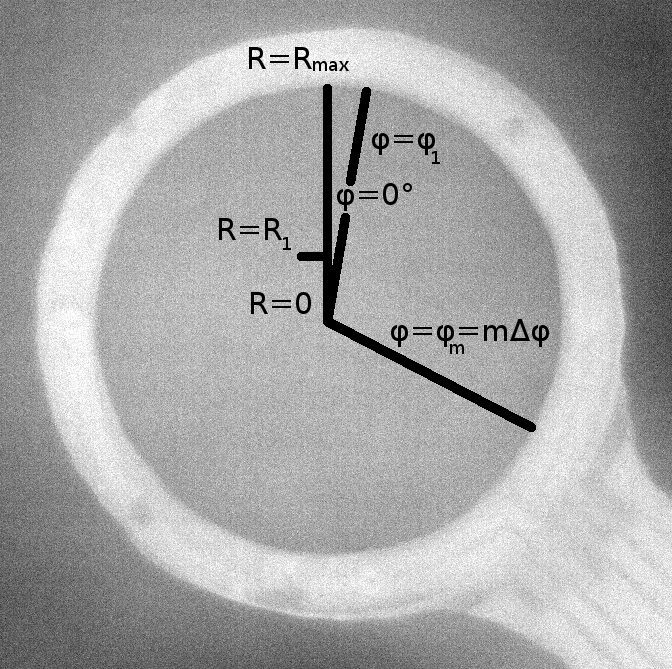
\includegraphics[width=0.4\textwidth,height=0.4\textwidth]{figs/auswertung/plasmaglw/randanalysemaske.png}
                  \caption{Schema der Maske für die Auswertung des Randschicht-Leuchtens (invertiert).}
                  \label{img:randmaske}
              \end{wrapfigure}

  Wie bereits erwähnt, erfolgte die Analyse des Plasma-Glow über die Aufsummierung der Intensitäten in einem selbst gewählten Bildbereich, welcher beliebig polar und radial unterteilt werden konnte. Aus dieser Summe wurde anschließend der Mittelwert der Intensität durch Division der Anzahl an Pixeln, mit einer Helligkeit $>0$ in dem jeweiligen Bereich, berechnet. \autoref{img:randmaske} zeigt, schematisch, die erstellte Maske für eine solche Auswertung. Der maximale Radius $R\ix{max}$ sollte dabei, günstiger Weise, immer noch vollständig innerhalb des Ringes liegen, damit keine falschen Helligkeitsinformationen hinzugezogen werden. Die Bildverarbeitung erfolgte nicht, wie es \autoref{img:glow} zeigt, sondern im invertieren Zustand. Dies hat zur Folge, das geringe Kontraständerungen als große Differenzen in den Intensitätswerten aufgenommen werden können. Insgesamt wurden 13 Messreihen von 2000 \tilt{frames} bei einer Bildrate von 200 \tilt{fps} aufgenommen, was demnach einer Messzeit von $\unit[10]{s}$ gleich kommt. Begonnen wurde mit einer Messung bei abgeschalteter Anregung bzw. einem \tilt{floatenden} Ring. Dazu kommen jeweils Aufnahmen von Anregungen einer Dipol-, Quadrupol- und Rotationsschwingung bei 3 sowie  $\unit[10]{Hz}$. Diese insgesamt 6 Messungen mit Anregung wurden danach, um noch genauer den Einfluss der Manipulation zu verstehen, für eine niedrigere Ring-Höhe (über der Thermophorese-Zelle) wiederholt. Zuerst betrug diese $\unit[1,8]{cm}$, dann $\unit[1,2]{cm}$. Die Aufnahmen wurden alle bei einem Gasdruck von $\unit[10,6]{Pa}$ und einer \tilt{rf}-Generator-Leistung von $\unit[1,6]{W}$ gemacht. Der relativ hohe Wert - bei Untersuchungen von Staub-Clustern lag dieser nur bei $\unit[0,5]{W}$ - wurde bewusst gewählt, da bei größeren Leistungen das Leuchten ebenso stärker wird. Dies ist u.a. eine Folge der erhöhten Elektronendichten. 

    \subsection{Messwerte}

        \begin{figure}[!t]
          \centering
          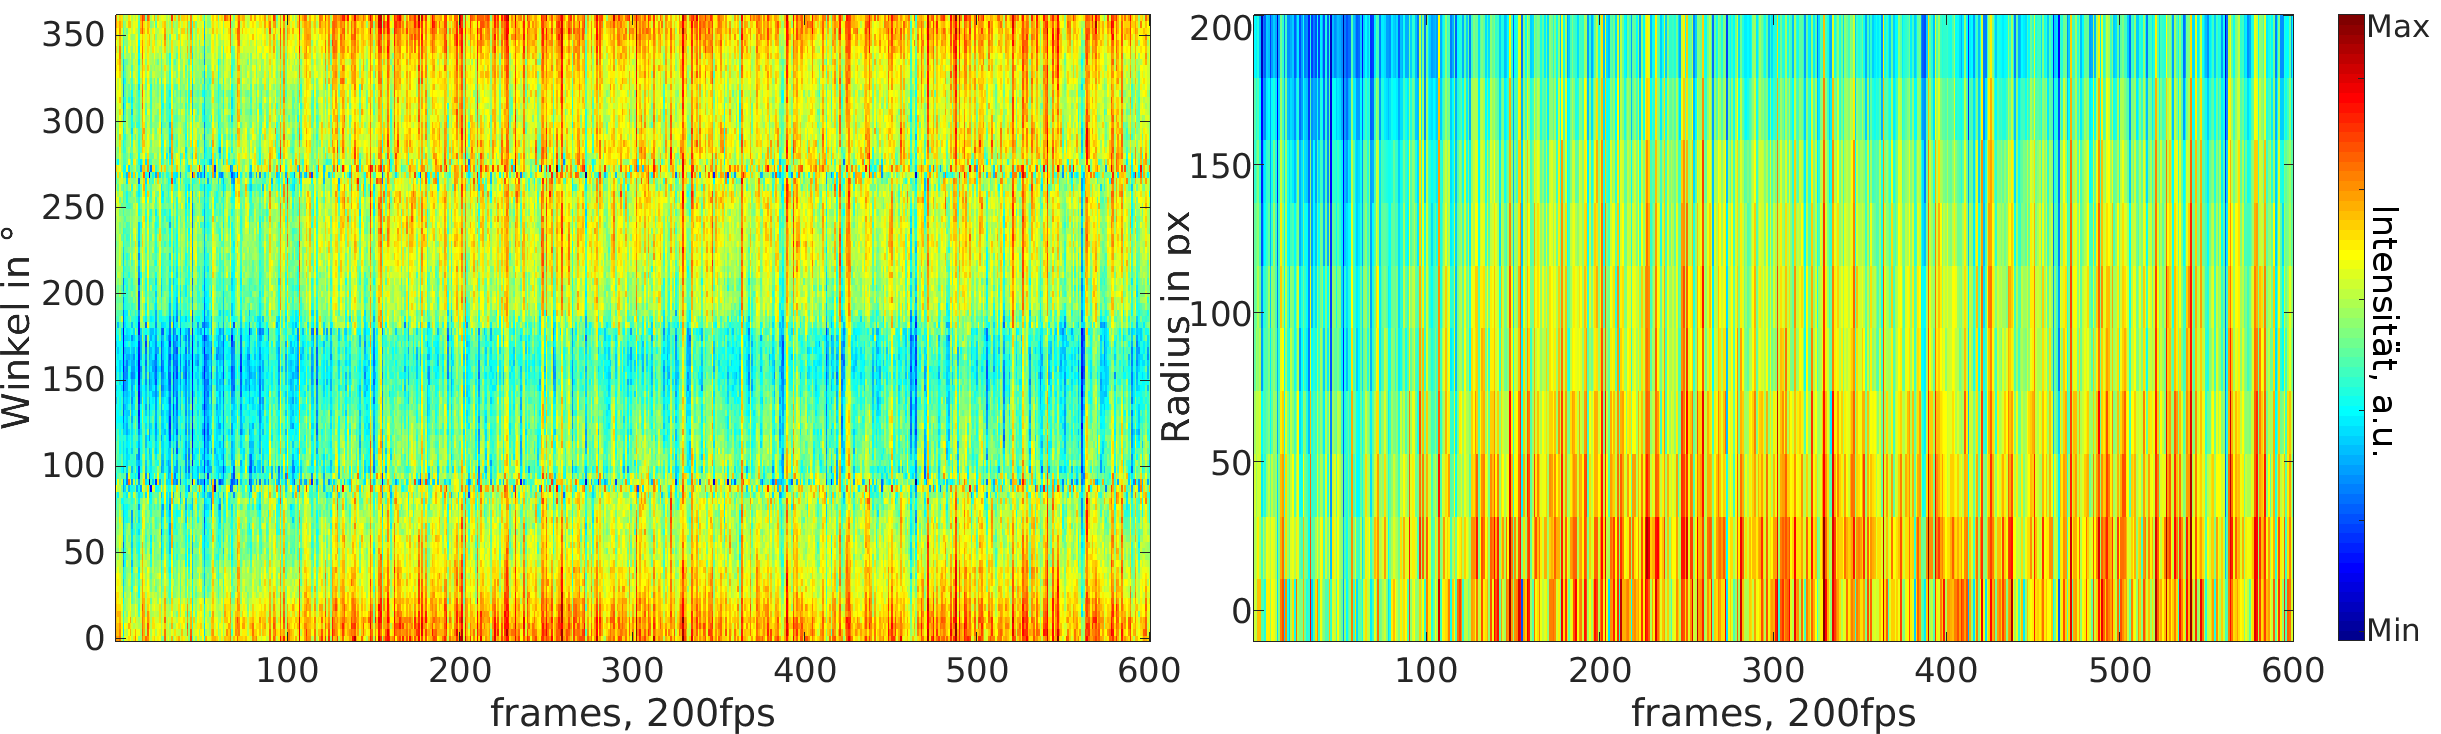
\includegraphics[width=\textwidth,,height=0.38\textwidth]{figs/auswertung/plasmaglw/randungest3sekwinkurad.png}
          \caption{\underline{\fett{links}:} Polar aufgelöster Intensitätsverlauf für eine Zeit von $\unit[3]{s}$ (600 \tilt{frames}) ohne Anregung. Die Intensität (siehe rechts) ist auf einen Durchschnittswert normiert. \underline{\fett{rechts}:} Die selbe Messung wie \underline{\fett{links}}, nur radial aufgelöst.}
          \label{img:randungest}
        \end{figure}

    In \autoref{img:randungest} sind die Daten der ersten Messung, in radialer und polarer (Winkel-) Auflösung, bei abgeschalteter Anregung und "`hoher"' Elektrode dargestellt. Zuerst fällt der Intensitätsabfall in der Winkeldarstellung bei $\varphi\approx\unit[140-180]{\degree}$ auf: dieser Bereich entspricht, nach \autoref{img:randmaske}, in etwa der Richtung des Arm der Elektrode. Dort ist das Plasma-Leuchten schwächer als am übrigen Ring. Hinzu kommt ein Helligkeits-Gradient von eben diesem Bereich in Richtung $\unit[0/360]{\degree}$. Das entspricht der gegenüberliegenden Seite des Rings. In radialer Darstellung zeigt sich, dass im Inneren der Elektrode, im Vergleich zu Außen, die Intensität wesentlich größer ist.\\
    Die \autoref{img:randfrequenz} stellt eine Dipol-Anregung bei den 2 unterschiedlichen Frequenzen dar (s.o.).  Sehr anschaulich und gut erkennbar sind die, sich abwechselnden, Maxi- und Minima der Intensität, welche mit der Frequenz der Anregung für einen Winkel (bspw. $\varphi=\unit[150]{\degree}$) "`durchschwingen"'. Im Bereich $\unit[50-220]{\degree}$ sind die Extrema sehr gut ausgeprägt, wohin gegen um $\unit[330]{\degree}$ der Kontrast zwischen den Schwingungszuständen sich weniger stark abzeichnet. Für eine höhere Frequenz der Manipulation verändert sich, bis auf die Zeitskalen der Variation der Helligkeiten, nichts.

      \begin{figure}[!b]
            \centering
            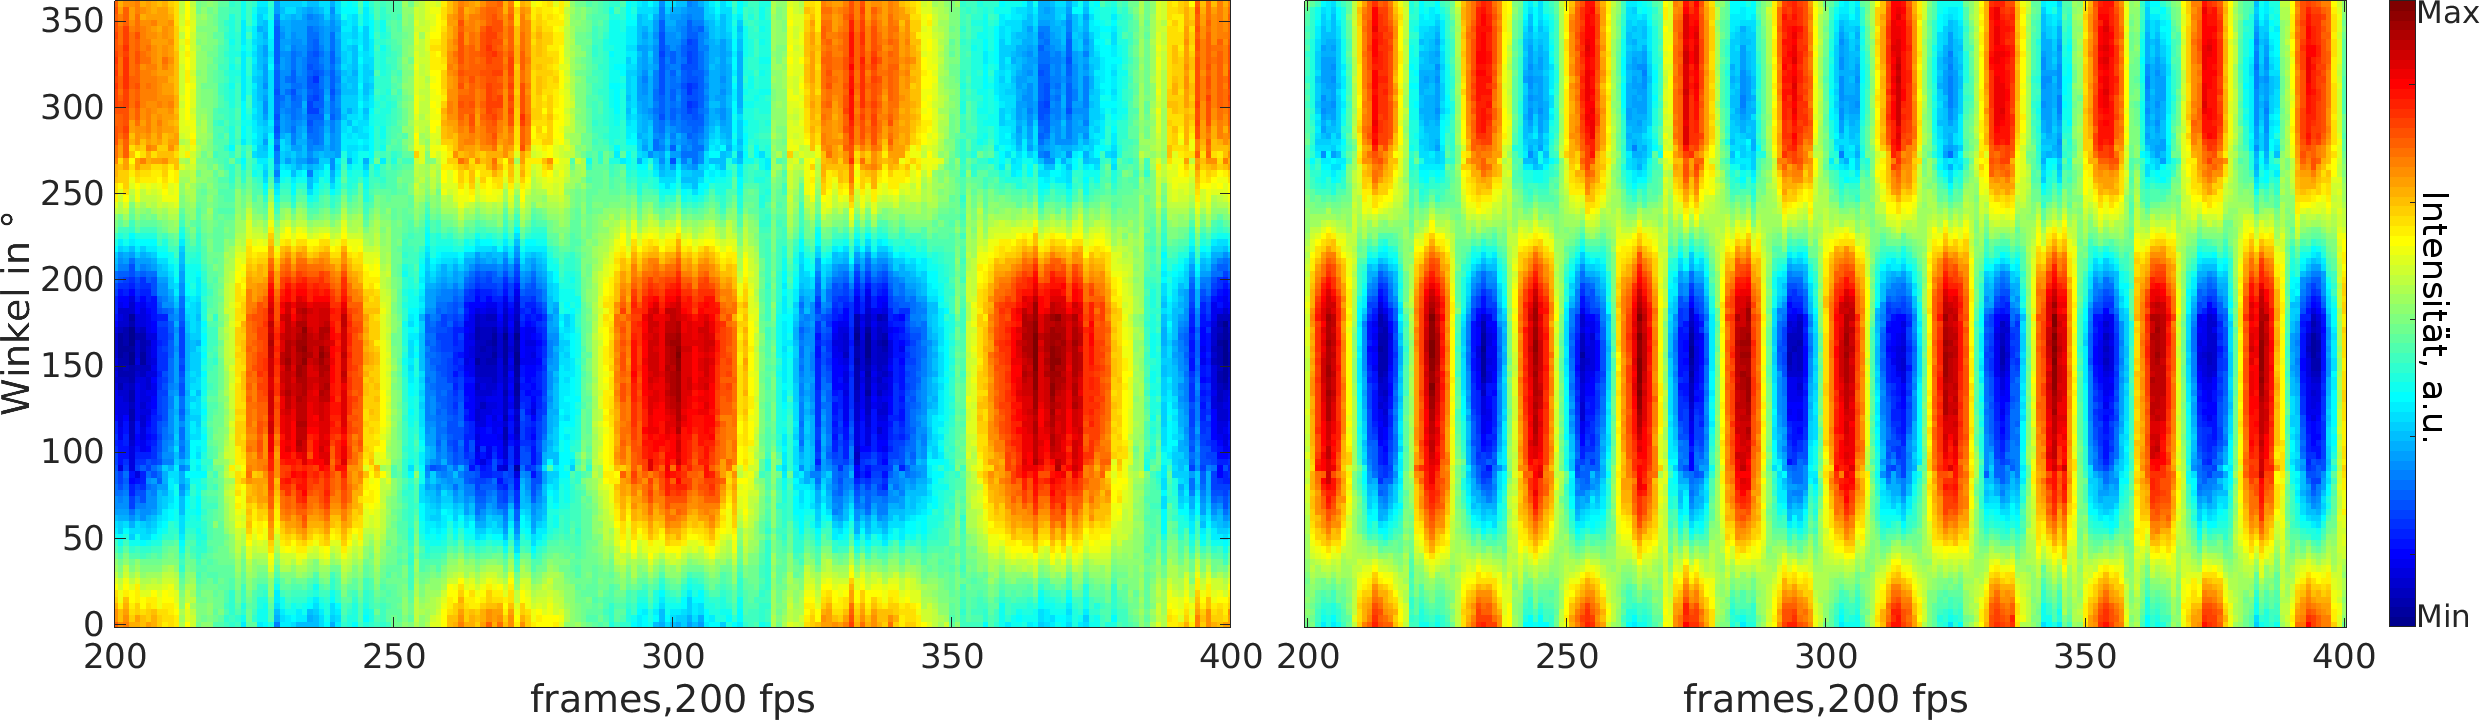
\includegraphics[width=\textwidth,height=0.38\textwidth]{figs/auswertung/plasmaglw/randdipol3hzu10Hz1sekwink.png}
            \caption{\underline{\fett{links}:} Winkeldarstellung der Dipol-Anregung bei $\unit[3]{Hz}$ für $\unit[1]{s}$. \underline{\fett{rechts}:} Bei $\unit[10]{Hz}$.}
            \label{img:randfrequenz}
      \end{figure}

      \begin{figure}[!t]
         \centering
         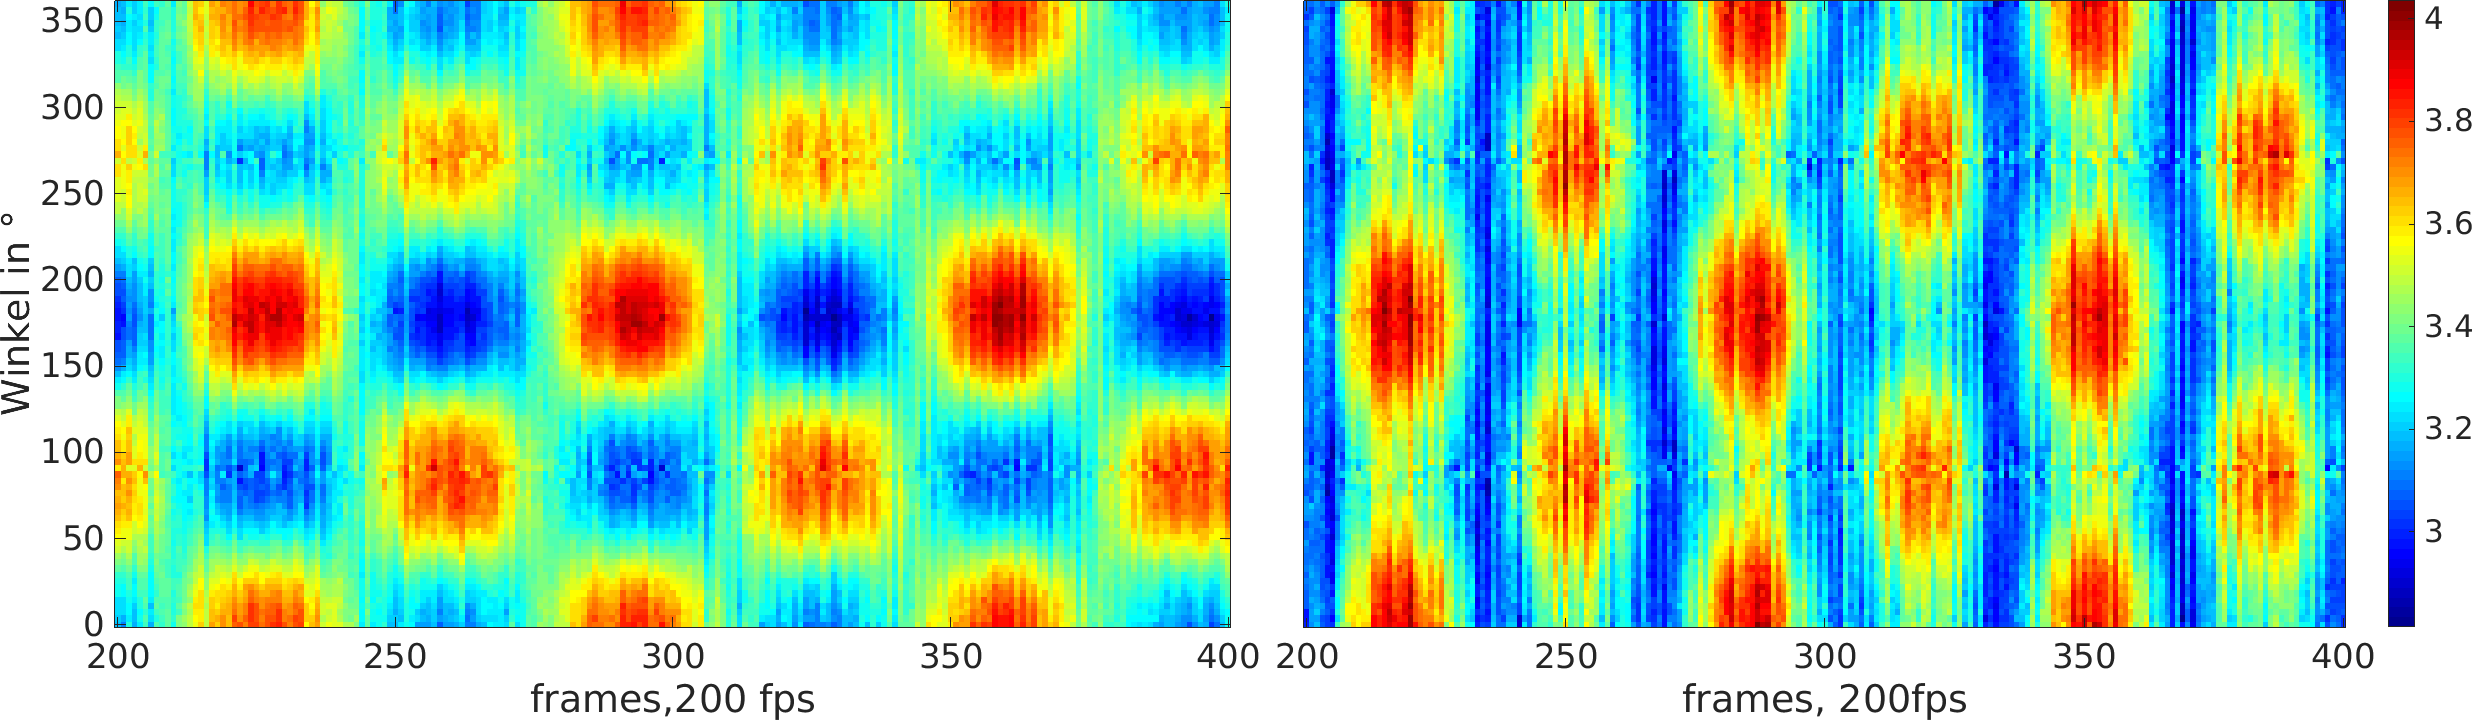
\includegraphics[width=\textwidth,,height=0.38\textwidth]{figs/auswertung/plasmaglw/randhochutiefquad3Hz1sekwink.png}
         \caption{Winkelaufgelöste Quadrupol-Anregung bei $\unit[3]{Hz}$. \underline{\fett{links}:} für eine Höhe von $\unit[1,8]{cm}$. \underline{\fett{rechts}:} Für $\unit[1,2]{cm}$.}
         \label{img:randhochutiefwink}
      \end{figure}

        In \autoref{img:randhochutiefwink} ist der Unterschied für die unterschiedlichen Höhen der Elektrode an einer Quadrupol-Anregung mit $\unit[3]{Hz}$ gezeigt. Bei einer Höhe von $\unit[1,8]{cm}$ (\autoref{img:randhochutiefwink}:\underline{\fett{links}}) fällt einerseits eine Asymmetrie zwischen den Maxima bzw. Minima einer Schwingungsachse auf. Jeweils 2, für einen Zeitschritt wie etwa für die \tilt{frames} 250 bis 275 zusammen auftretende, Extrema gehören zu einer Anregungsrichtung: zwischen $\unit[0/360]{\degree}$ und $\unit[180]{\degree}$, hier einmal $\Pi$ genannt, sowie $\unit[90]{\degree}$ und $\unit[270]{\degree}$, als $\Sigma$ bezeichnet. Andererseits - und dieser Unterschied ist wesentlich signifikanter - sind die Differenzen zwischen den Maxima und Minima der beiden Achsen. Die größten Intensitäten der Schwingungsrichtung $\Pi$ sind deutlich höher, als die der Achse $\Sigma$. Außerdem sind die Minima auf $\Sigma$ niedriger, als auf $\Pi$. In der Zeit, in welcher keiner der 4 Segmente eine Amplitude (max. oder min.) der Anregung trägt, zeichnet sich ein Übergang von einem Extremum zum anderen ab. Beispielsweise für die \tilt{frames} 335 bis 345 stellt sich im gesamten Ringbereich eine,näherungsweise gleiche Helligkeit ein.

      \begin{figure}[!b]
        \centering
        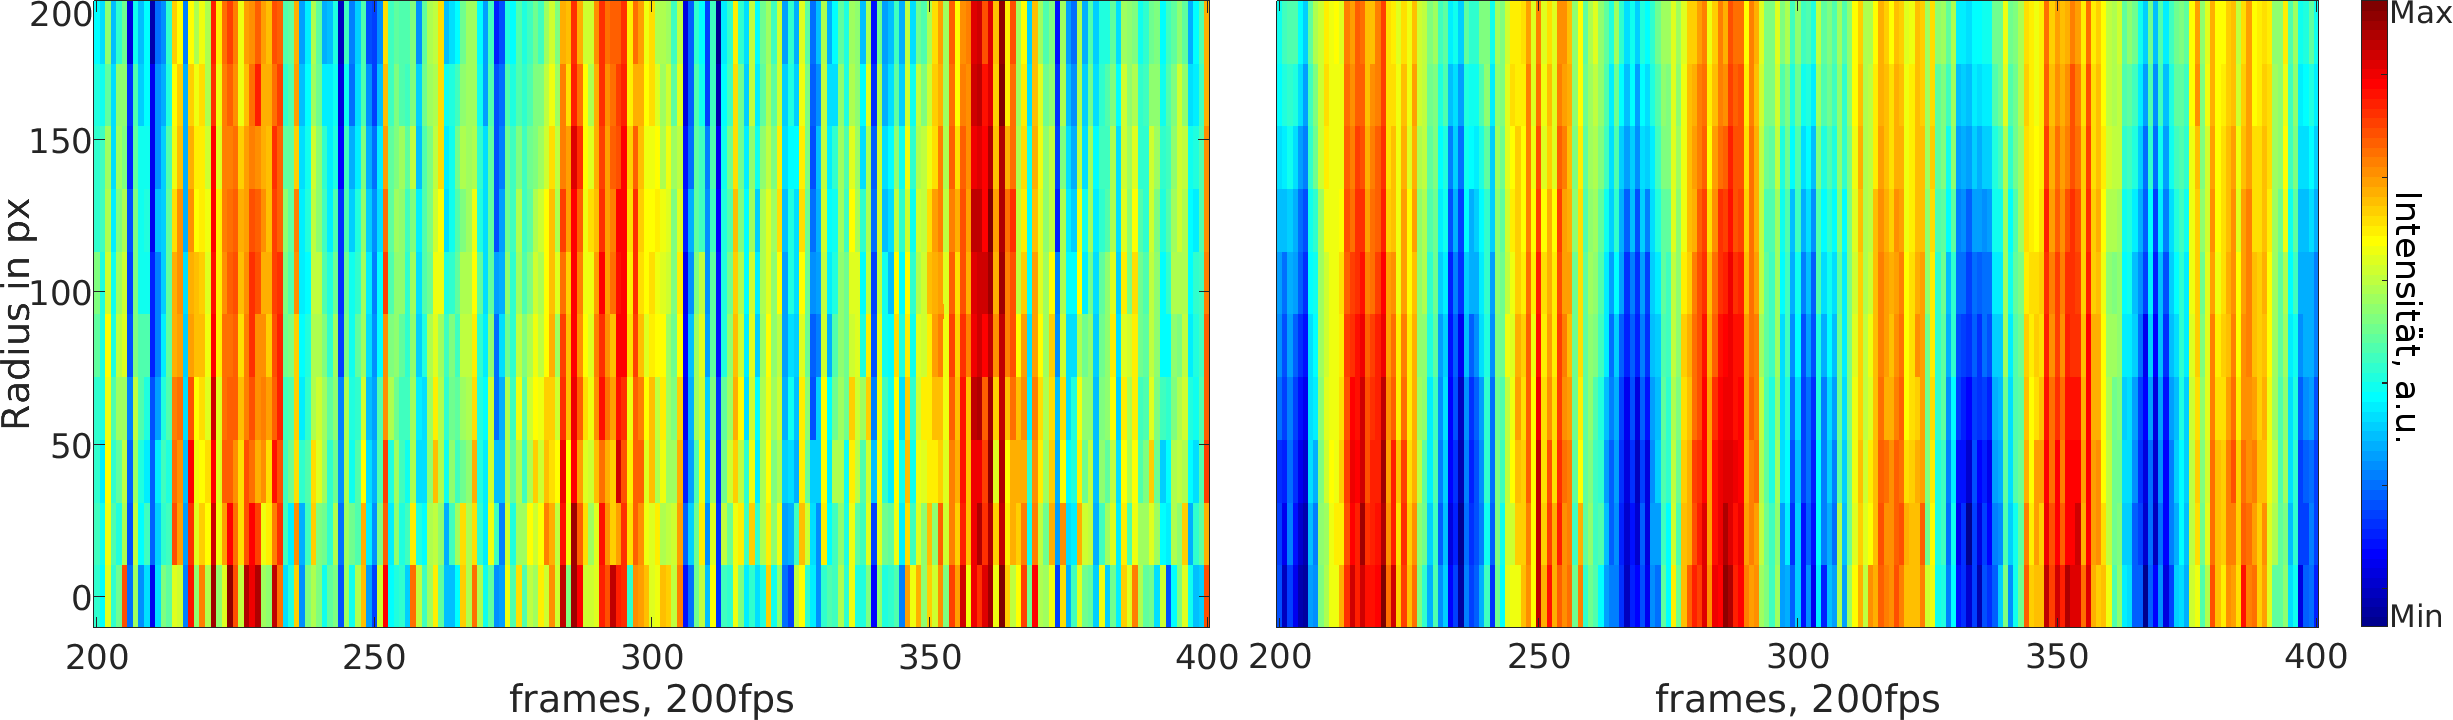
\includegraphics[width=\textwidth,height=0.38\textwidth]{figs/auswertung/plasmaglw/randhochutiefquad3Hz1sekrad.png}
        \caption{Radial aufgelöste Quadrupol-Anregung (selbige wie in \autoref{img:randhochutiefwink}) bei $\unit[3]{Hz}$. \underline{\fett{links}:} für eine Höhe von $\unit[1,8]{cm}$. \underline{\fett{rechts}:} Für $\unit[1,2]{cm}$.}
        \label{img:randhochutiefrad}
      \end{figure}

    Für eine niedriger angebrachte Elektrode (\autoref{img:randhochutiefwink}:\underline{\fett{rechts}}) findet man in etwa den gleichen Intensitätsverlauf wie zuvor. Es fallen Unterschiede sowohl zwischen den Maxima und Minima auf einer Schwingungsachse, als auch im Vergleich der beiden auf. Jedoch erkennt man weiterhin, im Kontrast zur Aufnahme bei einer hohen Elektrode, dass diese weniger scharf abgezeichnet sind. Das heißt: die Grenzen bzw. Übergänge der Extrema zwischen $\Sigma$ und $\Pi$ haben einen geringeren Intensitäts-Gradienten. Besonders gut ist dies im Bereich um \tilt{frame} 250 (und 100 \tilt{frames}-periodisch fortlaufend) zu erkennen - die Maxima dieser Phase der Anregung sind sehr verwaschen und verlaufen sich über den gesamten Winkelbereich. Jedoch zeichnet sich in den Momenten zwischen den Amplituden ein klares Tief in der Intensität ab, welches die Extrema unterschiedlicher Phasen der Anregung voneinander trennt. Für das Beispiel bei  \tilt{frame} 250 liegen diese zwischen \tilt{frame} 230 und 245, sowie 255 und 225. Demnach kann der Umschicht-Vorgang, welcher in \autoref{img:randhochutiefwink}:\underline{\fett{links}} als heller Übergang zwischen den Maxima der Achsen zu erkennen ist, im zeitlichen Verlauf nicht beobachtet werden. Lediglich gewinnen die Maxima auf $\Sigma$ geringfügig an Intensität, wohin gegen die Minima sowohl auf $\Sigma$ als auch $\Pi$ weniger ausgebildet sind.\\
    Die \autoref{img:randhochutiefrad} zeigt die exakt gleiche Messung wie die vorherige aus \autoref{img:randhochutiefwink}, nur in radialer Auflösung. Das linke Bild zeigt die Daten aus der Messung bei einer höheren Elektrode. Für die Zeiten um die \tilt{frames} 225, 290 und 360 ist jeweils das gesamte Innere des Ringes hell. Das heißt, dass über den gesamten radialen Bereich ein Maximum zu finden ist. Zwischen diesen können weitere erahnt werden. Jedoch sind diese Extrema, sowohl die maximalen als auch minimalen, sehr flach bzw. kaum erkennbar. Sie heben sich lediglich auf Grund der kleinen Bereiche um \tilt{frame} 210, 245, 275 310, 340 und 375 bei großen Radien, wie etwa $\unit[150-200]{px}$, von den übrigen Intensitäts-Maxima ab. Weiterhin ist insgesamt ein schwacher Gradient in der Helligkeit von innen $R=0$ bis $R=\unit[200]{px}$ zu erkennen.\\
    Bei einer tiefen Elektrode zeigt sich ein anderes Bild: alle Extrema sind scharf und eindeutig erkennbar. Für diese Einstellung zeigt sich die zuletzt benannte Diskrepanz zwischen den Schwingungsachsen nun wesentlich deutlicher. Demnach können die Schwingungen aus der vorherigen Beschreibung mit denen dieser Darstellung identifiziert werden. Das 1. Maximum gehört zu $\Pi$ und das 2. zu $\Sigma$ usw. Außerdem stellt man fest, dass die Helligkeit der Maxima von $\Sigma$ geringer ist, als die von $\Pi$. Interessant ist hingegen jedoch, dass die minimalen Intensitäten keine systematischen Differenzen mehr zueinander aufweisen. Für große Radien verschwimmen die Intensitäten und der Gradient nimmt, in Hinblick auf $R=0$, mit wachsendem Abstand zum Mittelpunkt zwischen den Extrema ab.

      \begin{figure}[!t]
        \centering
        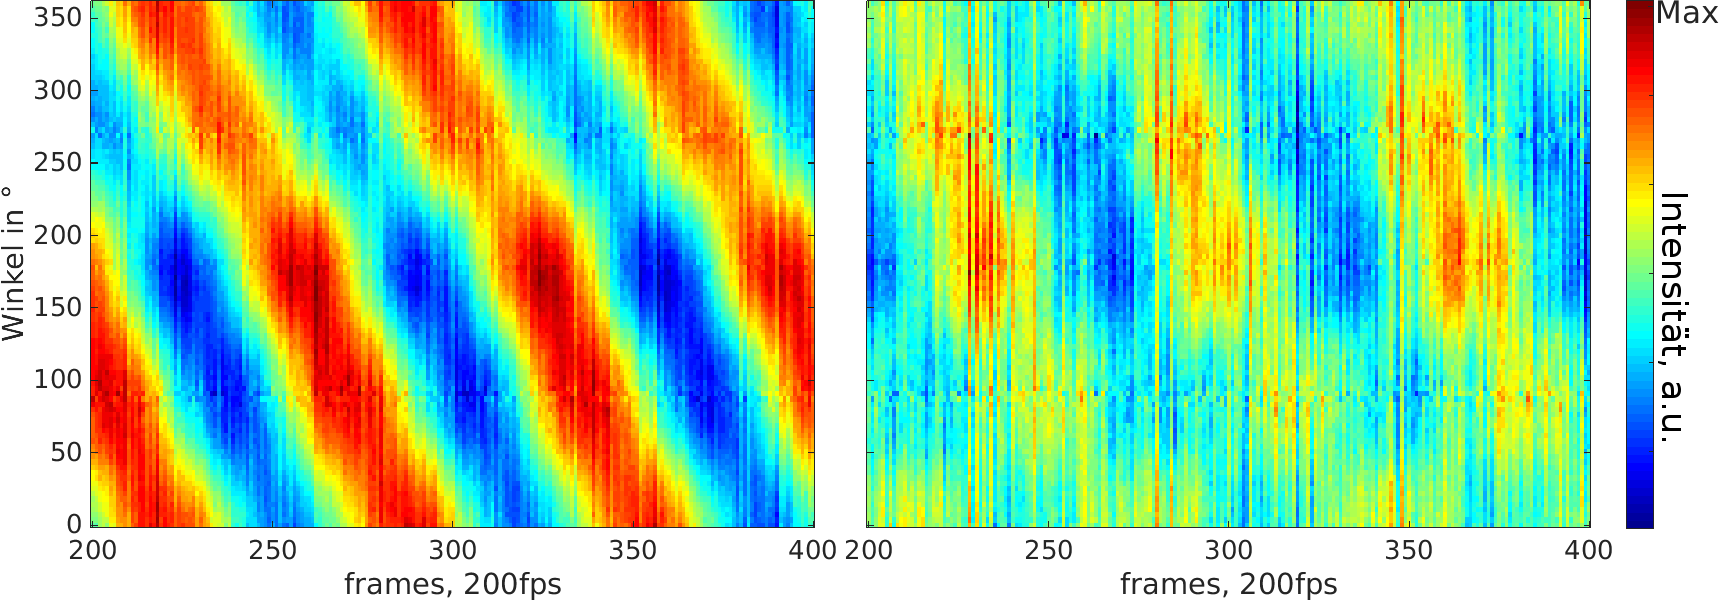
\includegraphics[width=\textwidth]{figs/auswertung/plasmaglw/randrotathochutief3Hz1sekwink.png}
        \caption{Intensitätsverlauf der Anregung einer Rotation bei $\unit[3]{Hz}$ und einer Zeit von $\unit[1]{s}$. \underline{\fett{links}:} Hohe Elektrode. \underline{\fett{rechts}:} Tief.}
        \label{img:randhochutiefrotat}
      \end{figure}

    Abschließend ist in \autoref{img:randhochutiefrotat} eine Rotations-Anregung mit Hilfe der Intensitätsanalyse visualisiert. Sehr anschaulich kann hier das Maximum bei seiner Wanderung von $\unit[360]{\degree}$, im Bereich um \tilt{frame} 235 (und um $200/3$ \tilt{frames} fortsetzend), über $\unit[180]{\degree}$ bei ca. \tilt{frame} 260 , bis hin zu $\unit[0]{\degree}$ bei \tilt{frame} 300 verfolgt werden. Im Zuge dessen können über das gesamte Winkelintervall mehr oder weniger stark ausgeprägte Inhomogenitäten der Intensität beobachtet werden: insbesondere bei $\unit[240-250]{\degree}$ ist ein stärkerer Abfall in der Helligkeit des Maximums zu vermerken. Um $\unit[180]{\degree}$ liegt die größte Intensität. Das Minimum zwischen den Bahnen der Rotationsanregung ist, bis auf eine Aufhellung und ein "`Verschmieren"' im Bereich des schwachen Maximums, gleichbleibend.\\
    Das rechte Bild der \autoref{img:randhochutiefrotat} zeigt die gleiche Anregung bei einer tiefen Elektrode. Der Verlauf des Helligkeits-Maximums ist beinahe vollständig unkenntlich geworden. Um $\unit[180]{\degree}$ ist wiederum die größte Intensität zu finden. Die, zwischen den, nunmehr kaum erkennbaren Bahnen liegenden Minima sind jetzt stark verschmiert und besonders in den Bereichen um $\unit[360]{\degree}$ nicht vom Rest unterscheidbar. Interessant ist jedoch, dass sich etwas ähnliches wie \tilt{hot-spots} des Leuchtens ausbilden: bei $\unit[90]{\degree}$ und \tilt{frame} 250 , $\unit[0]{\degree}$ und  \tilt{frame} 275 sowie $\unit[270]{\degree}$ und \tilt{frame} 225 finden sich, aus dem verbliebenen Verlauf der Rotation herausstechende Intensitäten. 

    \subsection{Auswertung}

        \begin{figure}[!b]
          \centering
          \hspace{-0.7cm}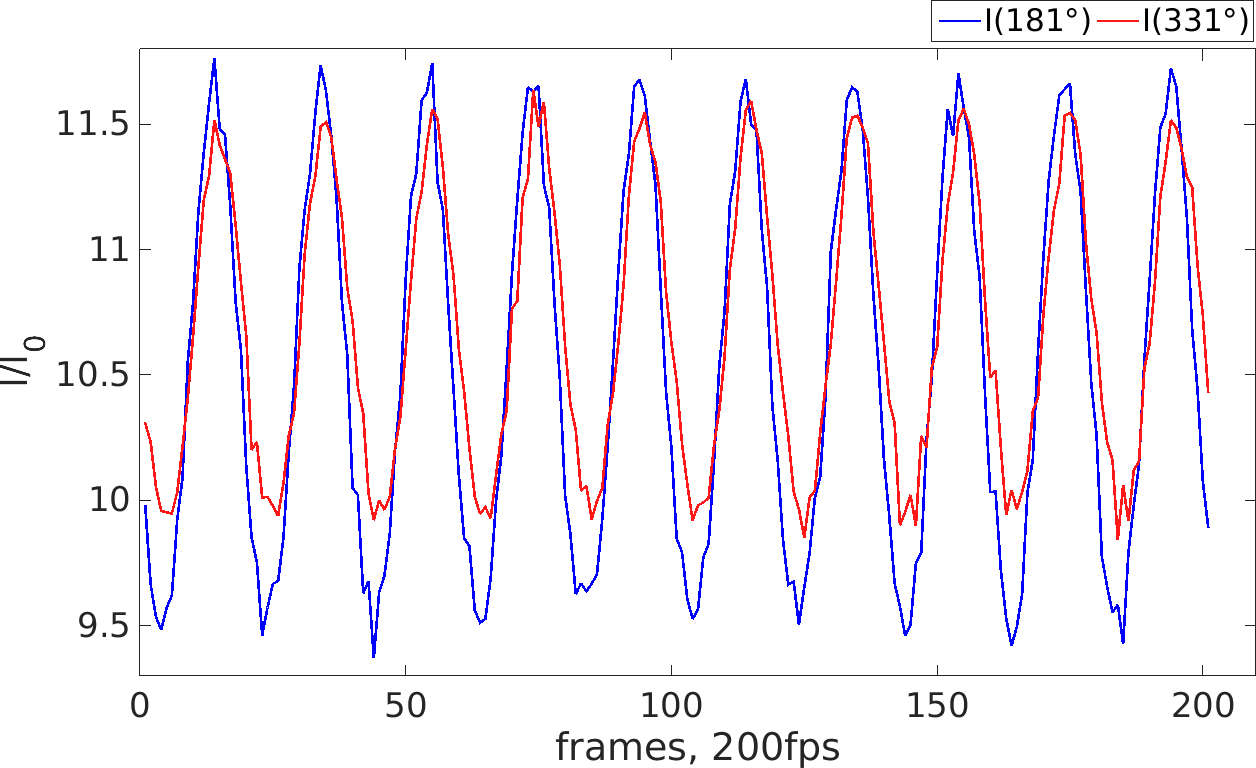
\includegraphics[width=0.65\textwidth,height=0.4\textwidth]{figs/auswertung/plasmaglw/intensdipol181u3313Hz1sek.png}
          \caption{Vergleich der Intensitätsverläufe bei $\unit[149]{\degree}$  und $\unit[331]{\degree}$ der Dipol-Anregung von \autoref{img:randfrequenz} bei $\unit[3]{Hz}$ für $\unit[1]{s}$. $I\left(\varphi=\unit[331]{\degree}\right)$ ist um 33 \tilt{frames} verzögert, damit die Extrema übereinander liegen.}
          \label{img:intensdipol}
        \end{figure}

      Mit den Ergebnissen der \autoref{img:randfrequenz} bis \autoref{img:randhochutiefrotat} ist die Methodik der Versuche um das Plasma-Glow prinzipiell bestätigt. Die Potentiale auf der Ring-Elektrode beeinflussen die Randschicht in dessen näherer Umgebung. Das kann man der lokalen Veränderung des Leuchtens in Folge der Manipulation entnehmen. Diese Einflüsse sind nur auf Zeitskalen der Cluster-Dynamik (Sekunden, Herz) und den räumlichen Dimensionen des Ringes (Zentimeter) von Bedeutung. Das Verhalten der Rand- bzw. Vorschicht während der \tilt{rf}-Zyklen spielte keine Rolle in den vorher gemachten Beobachtungen. Es kann demnach gefolgert werden, dass durch die Anregung mit der segmentierten Elektrode das lokale Potential verändert wird. Insbesondere kann daraus geschlossen werden, dass die Manipulation eines Yukawa-Clusters eindeutig durch die elektrostatische Wechselwirkung direkt mit dem Ring und dem abgewandelten Einfang erfolgt. Auf Grundlagen dessen sollen nun konkrete Analysen und Interpretationen vorgenommen werden.

      \paragraph{Dipol-Anregung}

          \begin{figure}[!t]
            \centering
            \begin{subfigure}{0.49\textwidth}
              \centering
              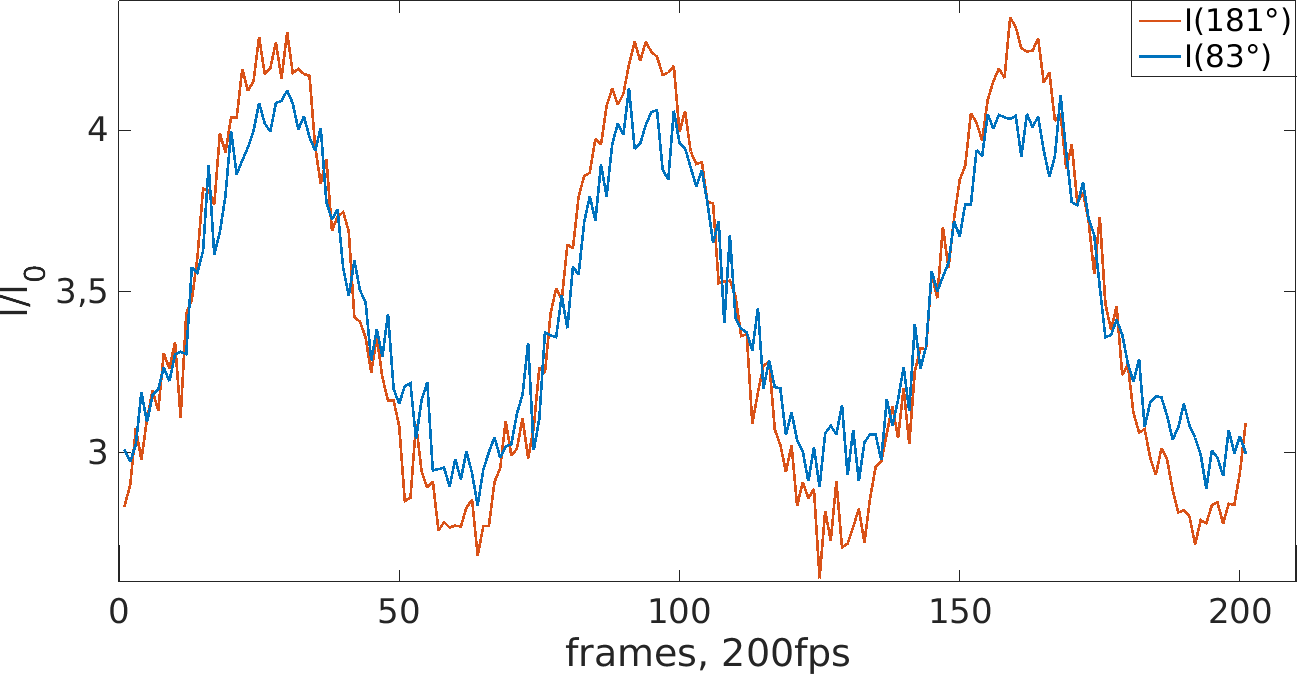
\includegraphics[width=\textwidth,height=0.65\textwidth]{figs/auswertung/plasmaglw/intens83u180quadinphase3Hz1sek.png}
            \end{subfigure}
            \begin{subfigure}{0.49\textwidth}
              \centering
              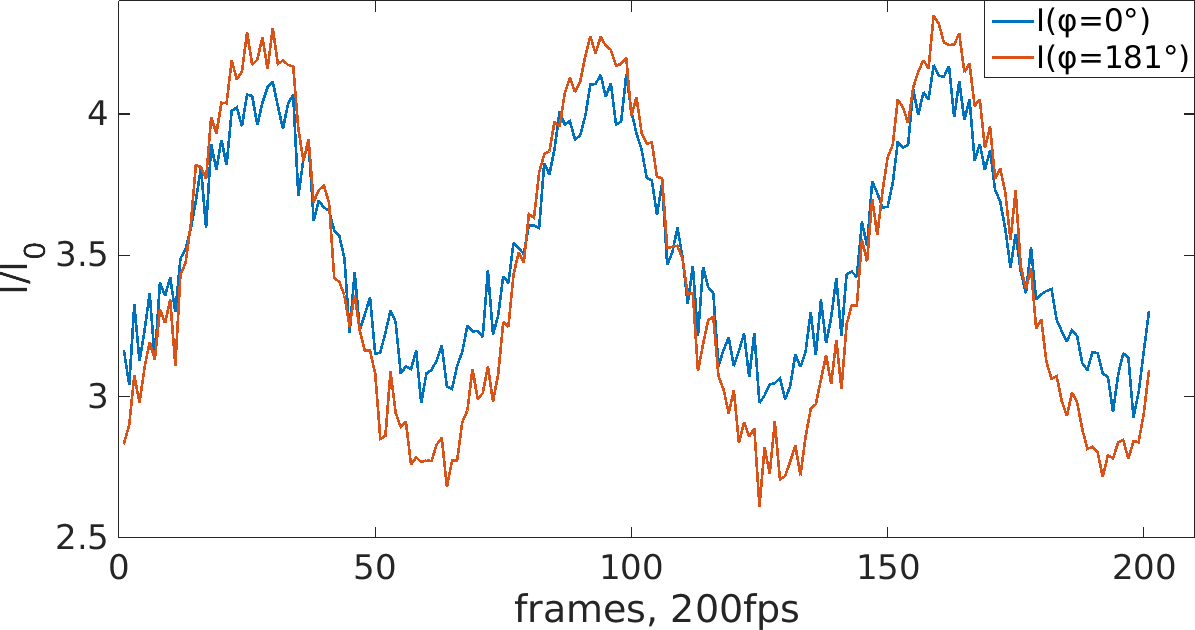
\includegraphics[width=\textwidth,height=0.65\textwidth]{figs/auswertung/plasmaglw/intens0u180quad3Hz1sek.png}
            \end{subfigure}
            \caption{Intensitätsverläufe der Quadrupol-Anregung aus \autoref{img:randhochutiefwink}:\underline{\fett{links}} bei $\unit[3]{Hz}$ für $\unit[1]{s}$. \underline{\fett{links}:} Bei $\unit[181]{\degree}$ und $\unit[83]{\degree}$. $I\left(83\degree\right)$ ist um 33 \tilt{frames} verzögert. \underline{\fett{rechts}:} Für $\unit[181]{\degree}$  und $\unit[0]{\degree}$. }
            \label{img:intensquadhochwink}
          \end{figure}

        Die für \autoref{img:randfrequenz} besprochenen Unterschiede zwischen den Extrema der beiden Pole lassen sich leicht in einem direkten Vergleich ablesen. Dabei werden die zeitlichen Verläufe der Helligkeit der Winkel $\unit[149]{\degree}$, genannt $\Phi$, und $\unit[331]{\degree}$, als $\Theta$ bezeichnet, mit ihren Maxima und Minima übereinander gelegt, damit direkt die Differenzen eingesehen werden können. In \autoref{img:intensdipol} ist , für das gleiche Zeitintervall wie es in \autoref{img:randfrequenz} dargestellt wurde, dieser Vergleich vorgenommen worden. Man erkennt leicht die Unterschiede zwischen den Amplituden der Intensität: sowohl maximale als auch minimale Helligkeit in Richtung von $\Phi$ sind stärker ausgebildet als die von $\Theta$. Diese Differenz beträgt im Mittel 3\%. Jedoch sind die Unterschiede zwischen den Minima größer als die der Maxima.\\
        Vergleicht man die Winkelanordnung der zwei benannten Pole mit der Maske aus \autoref{img:randmaske}, so sieht man, dass diese, ebenso wie bei einem "`echten"' Dipol, 2 gegenüberliegenden Segmenten des Ringes entsprechen. Diese Feststellung ist in Einklang mit den Erwartungen an diese Untersuchung. Hingegen weniger diesen entsprechend, ist die Differenz zwischen den Extrema der Intensität, welche zu jeweils 2 zusammen gelegten Segmenten gehörten. Wie bereits erwähnt, manipuliert der Pol $\Phi$ den Glow in seiner Umgebung stärker als $\Theta$. In der Richtung von $\Phi$ findet sich außerdem der Arm der Ring-Elektrode. Dessen Randschicht ragt in den Ring hinein und geht in die anliegenden Segmente über. Die Vermutung ist nun, dass sich deswegen die Randschichten der umliegenden Segmente und deren Glow verändert. Auf diese Weise kann besonders gut die stärkere Ausprägung der Minima von $\Phi$ erklärt werden. Andererseits beschreibt diese theorie nicht, warum ebenso in den Maxima ein signifikanter Unterschied besteht. Eine Möglichkeit das zu erklären ist, dass die Isolierung der Befestigung nicht lückenlos bzw. der Ring nicht vollkommen symmetrisch war. Demnach handelt es sich bei dieser Inhomogenität um einen systematischen Fehler.

          \begin{figure}[!b]
            \centering
            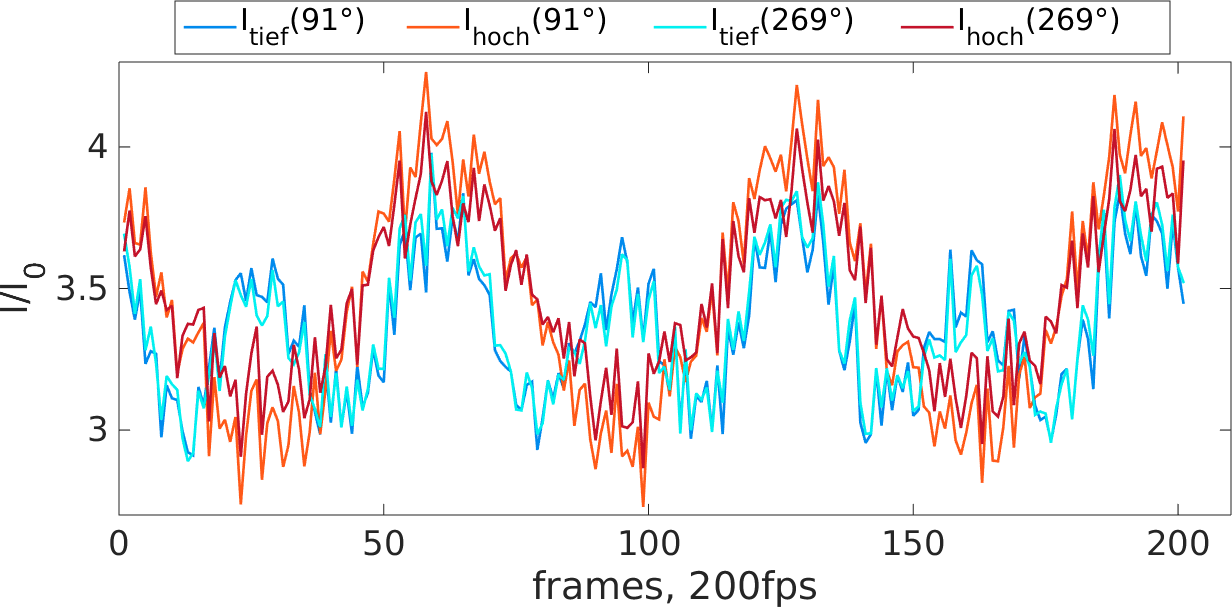
\includegraphics[width=0.8\textwidth,height=0.45\textwidth]{figs/auswertung/plasmaglw/intens270u90hochutiefquad3Hz1sek.png}
            \caption{Intensitätsverläufe bei $\unit[91]{\degree}$ und $\unit[269]{\degree}$ der Quadrupol-Anregung aus \autoref{img:randhochutiefwink} für einen hohen und tiefen Ring, bei $\unit[3]{Hz}$ für $\unit[1]{s}$. }
            \label{img:intensquadhochutief}
          \end{figure}

      \paragraph{Quadrupol-Anregung}

        Für den Verlauf der Helligkeit aus \autoref{img:randhochutiefwink}:\underline{\fett{links}} \autoref{img:intensquadhochwink} die, analog zur Analyse der Dipol-Schwingung, entsprechende Grafik. Für die beiden Vergleiche - einerseits zwischen den Achsen $\Sigma$ und $\Pi$ in \autoref{img:intensquadhochwink}:\underline{\fett{links}}, als auch für eine Achse $\Pi$ in \autoref{img:intensquadhochwink}:\underline{\fett{rechts}} - zeigen sich ähnliche Verhältnisse wie im vorherigen Abschnitt. In Richtung des Elektroden-Armes um $\varphi\approx\unit[150]{\degree}$ findet man allgemein stärkere Extrema vor. Konkret liegen die Intensitäten 3\%-5\% auseinander. Was jedoch die Vermutung der Beeinflussung der Randschicht durch den Ausleger bestätigt, ist der Unterschied zwischen den Differenzen in den beiden Bildern: für $I(\varphi=\unit[83]{\degree})$ finden sich näherungsweise gleiche Minima wie für $I(\varphi=\unit[181]{\degree})$. Dies ist jedoch nicht der Fall bei $I(\unit[0]{\degree})$. Des Weiteren kann auch die Vermutung über die Inhomogenität bekräftigt werden. Da bei der Quadrupol-Anregung jedes Segment um jeweils $\unit[90]{\degree}$ in der Phase verschoben war, sind die Extrema diesen eindeutig zuzuordnen. Daher kann aus den Unterschieden der vergleichenden Graphen auf die Asymmetrie des Ringes bzw. Fehler in der Fertigung dessen geschlossen werden.

          \begin{figure}[!t]
            \centering
            \begin{subfigure}{0.49\textwidth}
              \centering
              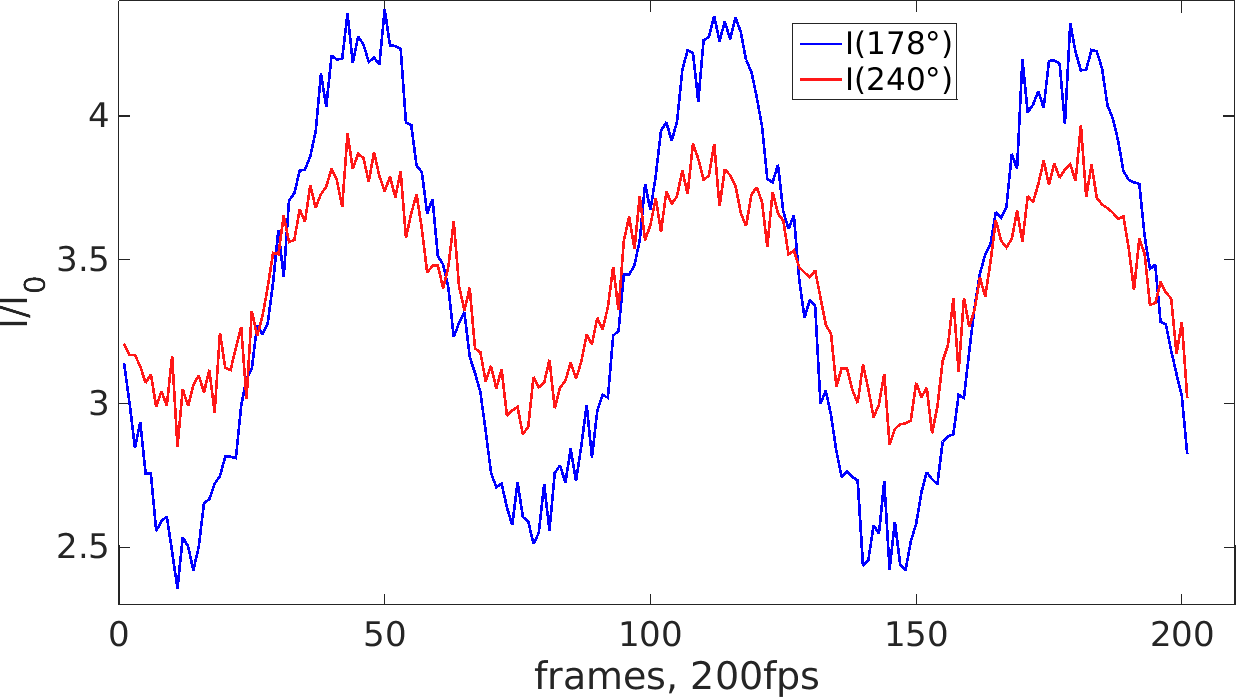
\includegraphics[width=\textwidth,height=0.65\textwidth]{figs/auswertung/plasmaglw/intensrotathoch178u2402Hz1sek.png}
            \end{subfigure}
            \begin{subfigure}{0.49\textwidth}
              \centering
              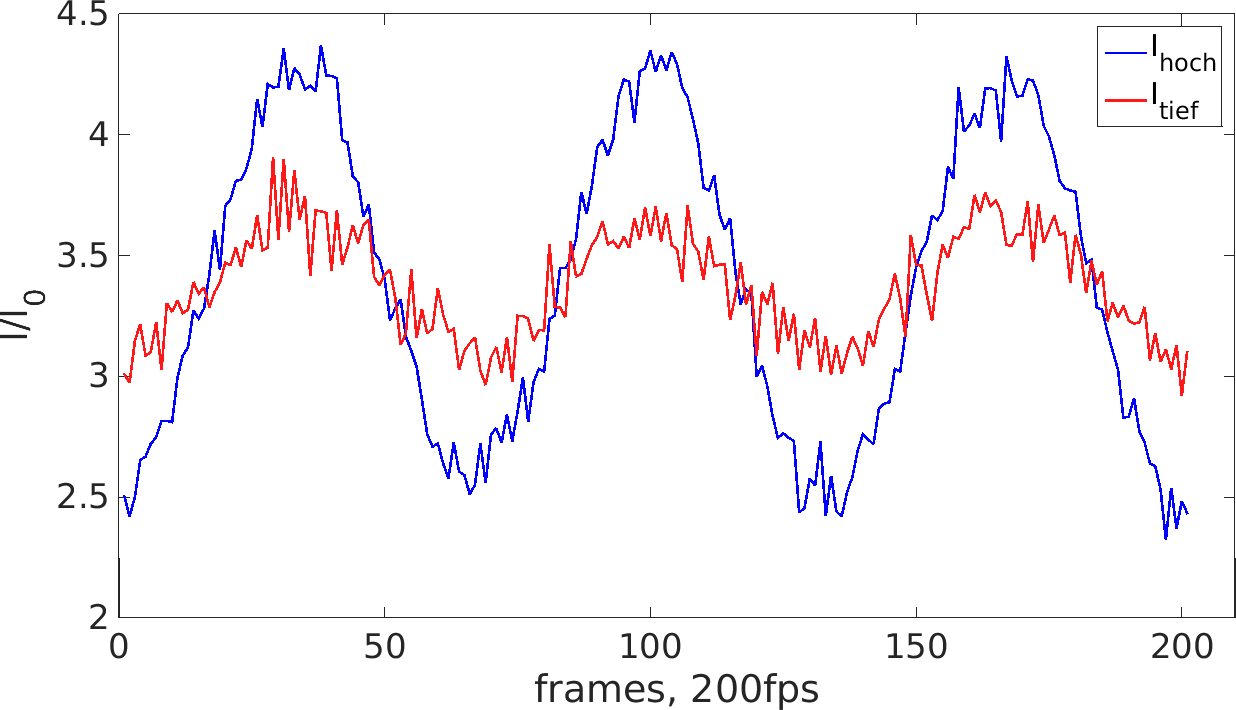
\includegraphics[width=\textwidth,height=0.65\textwidth]{figs/auswertung/plasmaglw/intensrotathochutief1783Hz1sek.png}
            \end{subfigure}
            \caption{Intensitätsverläufe einer Rotations-Anregung bei $\unit[3]{Hz}$ für $\unit[1]{s}$. \underline{\fett{links}:} Vergleich zweier Richtungen bei hoher Ring-Elektrode. $I\left(178\degree\right)$ ist um 33 \tilt{frames} verzögert. \underline{\fett{rechts}:} Für einen Winkel für unterschiedliche Höhen.}\label{img:intensrotathochutief}
          \end{figure}

          \begin{figure}[!b]
            \centering
            \begin{subfigure}{0.49\textwidth}
              \centering
              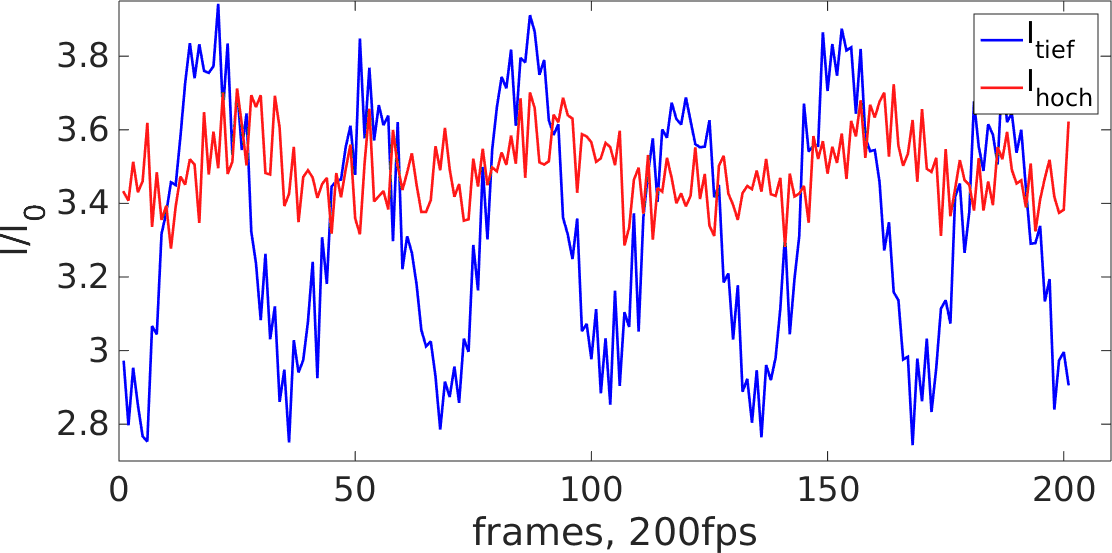
\includegraphics[width=\textwidth,height=0.65\textwidth]{figs/auswertung/plasmaglw/intenshochutiefquadin3Hz1sek.png}
            \end{subfigure}
            \begin{subfigure}{0.49\textwidth}
              \centering
              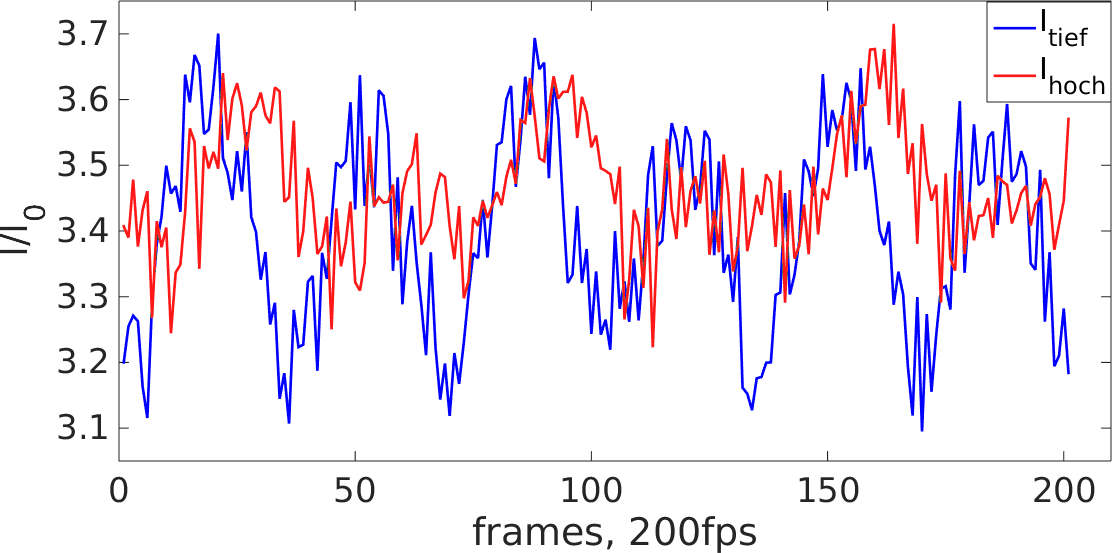
\includegraphics[width=\textwidth,height=0.65\textwidth]{figs/auswertung/plasmaglw/intenshochutiefquadout3Hz1sek.png}
            \end{subfigure}
            \caption{Intensitätsverläufe einer Quadrupol-Anregung bei $\unit[3]{Hz}$ für $\unit[1]{s}$. \underline{\fett{links}:} Vergleich hoher und tiefer Elektrode bei $R=0$. \underline{\fett{rechts}:} Für $R=R\ix{max}$.}\label{img:intensquadhochutiefrad}
          \end{figure}

        Mit \autoref{img:intensquadhochutief} schließt sich der Vergleich zweier ausgewählter Richtungen (Segment 4 und 2) für unterschiedliche Ring-Höhen an. Deutlich erkennt man die insgesamt niedrigere Intensität für einen tiefen Ring. Auch ist die verschwindend geringe Differenz zwischen den Intensitäten der gegenüberliegenden Segmente auffällig. Das ist in Einklang mit den vorherigen Ausführen. Eine Überraschung stellt jedoch das zusätzliche Maximum dar, welches an Stelle der Minima der Graphen für eine hohe Elektrode auftaucht. Dieses wurde bereits in \autoref{img:randhochutiefwink}:\underline{\fett{rechts}} beobachtet und kann somit hier bestätigt werden. Hängt der Ring nahe genug über der Elektrode (einer Metalloberfläche), so kann eine Oszillation des Glows mit der doppelten Frequenz der Anregung in der Mitte des Ringes beobachtet werden. Bei der Quadrupol-Anregung liegen dementsprechend, während einer Periode zwei mal, gleichzeitig Maxima und Minima auf den Segmenten der beiden Schwingungsachsen. Darauf baut die Vermutung auf, dass die Randschicht-Verformung dieser Potentiale groß genug ist, damit auch die Ring-Mitte dunkel wird. Das manifestiert sich als Minimum (in \autoref{img:randhochutiefwink}:\underline{\fett{rechts}}) vor und nach dem neuen Maximum (\autoref{img:intensquadhochutief}). Liegen wiederum nur schwache oder keine Potentiale auf den Segmenten, so kehrt das Plasma innerhalb des Ringes in den Ausgangszustand zurück und es kann wieder das Leuchten beobachtet werden. Die Schwingung des Plasma-Glow in der Mitte hat gerade die doppelte Frequenz der Anregung. Diese Beobachtung bzw. Entdeckung wird im weiteren Verlauf der Auswertung eine wichtige Rolle spielen, da sie mit dieser Art der Manipulation nicht beabsichtigt war.\\
        Die \autoref{img:intensquadhochutiefrad} zeigt Vergleiche der Intensitätsverläufe bei hoher und niedriger Elektrode für die Mitte $R=0$ und den Rand des Ringes $R=R\ix{max}$. Die Daten der Graphen entsprechen denen der Darstellung aus \autoref{img:randhochutiefrad} sowie \autoref{img:randhochutiefwink}. In den beiden Grafiken sind nochmals, gut deutlich, die Kontraste zwischen den sehr scharfen Extrema einer niedrig angebrachten Anregung und der verschmierten Verteilung der Helligkeit eines hohen Ringes zu sehen. Insbesondere können damit die vorher nur zu erahnenden Maxima bestätigt werden, sind sie dennoch verschwindend klein. Wiederum ist die Intensität bei einer niedrigen Höhe für die entsprechenden Minima wesentlich geringer. Es finden sich zudem 6 Extrema bei einer Anregung von $\unit[3]{Hz}$: das Leuchten innerhalb des Ringes schwingt mit. Beim maximalen Radius sind hingegen die Extrema von $I\ix{tief}$ weniger und die von $I\ix{hoch}$ stärker ausgeprägt. Das ist Folge der Nähe zur Quelle der Anregung. Durch das Mitteln über ein Radius-Intervall und einen vollen Winkelbereich, gehen in die Intensität des letzten Abschnitts sowohl dunkle Randschichten als auch helles Glow mit ein. Direkt an den Segmenten geschehen demnach signifikante Veränderungen der Grenzschicht des Plasmas, was mit dem Konzept des Ringes in Einklang ist.

      \paragraph{Rotations-Anregung}

        Abschließend erfolgt eine Betrachtung der Intensitäten bei einer Rotations-Anregung. Hierbei werden einerseits in \autoref{img:intensrotathochutief}:\underline{\fett{links}} die, für \autoref{img:randhochutiefrotat} besprochenen, charakteristischen Winkel bei denen Inhomogenitäten auftraten, verglichen. Andererseits zeigt \autoref{img:intensrotathochutief}:\underline{\fett{rechts}} den Verlauf der Helligkeit des selben Winkelelements bei verschiedenen Ring-Höhen. Die erste Grafik gibt deutlich die Asymmetrien der Segmente 1 und 3 wieder, wie sie zuvor mehrmals beobachtet wurden. Die Differenz in der Intensität liegt im Mittel zwischen 7\% und 8\%. Der zweite Vergleich zeigt die schwachen Extrema einer Rotation bei einem kleinen Abstand zur Randschicht der Elektrode. Da bei dieser Anregung jeweils nur eines der Segmente ein minimales Potential tr\"agt, w\"ahrend die anderen schwach negative bzw. maximale haben, ist der Intensitätsverlauf innerhalb des Ringes nicht-trivial. Im Bereich um das Element mit dem kleinsten Potential ist der Glow, auf Grund der in diesem Augenblick Massepotential tragenden angrenzenden Segmente, stark verändert. Das \"ubrige Segment hat zu dieser Zeit ein Maximum und zeigt das, zum Minimum umgekehrte Verhalten. Insgesamt ist das, auf einer Ring-Bahn ``wandernde'' Leuchten (bzw. Dunkel) wesentlich kontrast\"armer. Die \tilt{hot-spots} aus \autoref{img:randhochutiefrotat} k\"onnen, mit der gewonnenen Kenntnis, in etwa als die Mittelpunkte der Segmente identifiziert werden, was nahe legt, dass dort die Glow-Manipulation am st\"arksten ist. Jedoch spricht dies nicht f\"ur die Qualit\"at des Ringes als symmetrische Multipol-Elektrode. Insbesondere findet kann stetiger Übergang zwischen den Segmenten statt, da dort ein etwa $\unit[1]{mm}$ breiter Bereich ohne Kupfer frei liegt.

%						\begin{figure}[!t]
%							\centering
%							\begin{subfigure}{0.49\textwidth}
%								\centering
%								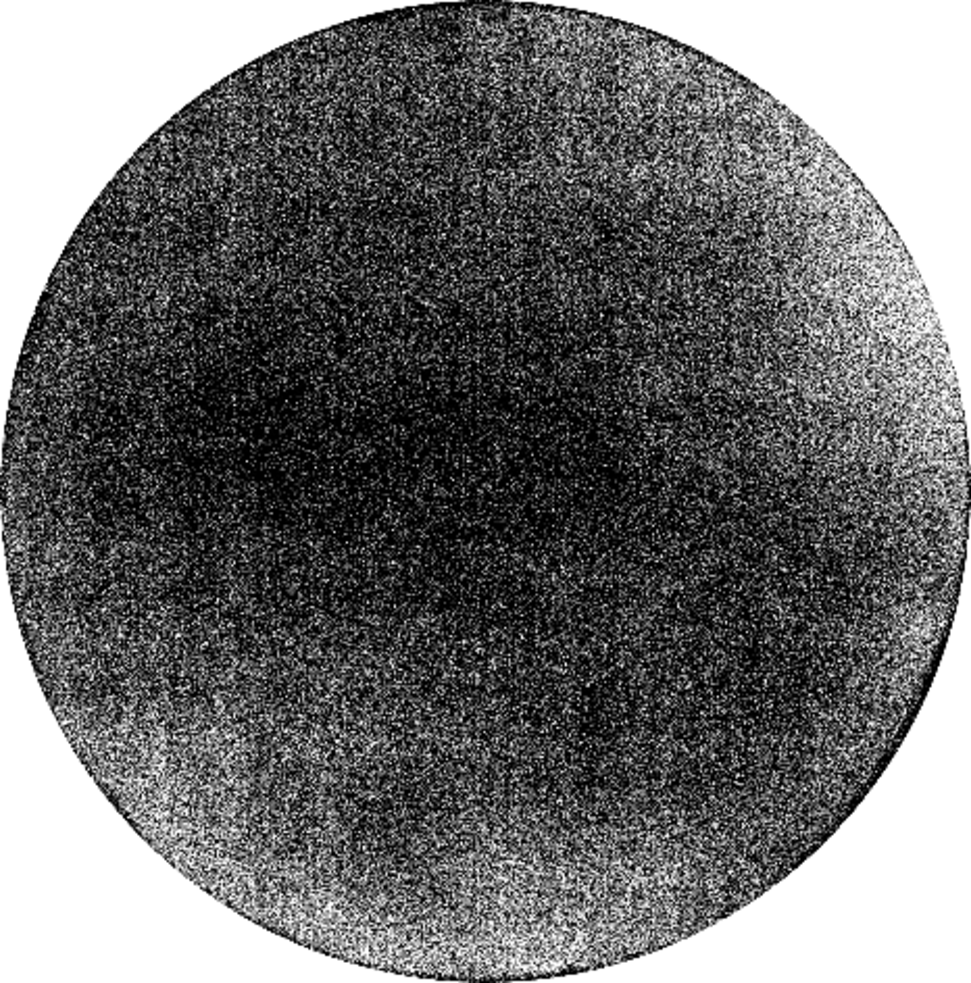
\includegraphics[width=0.5\textwidth,height=0.5\textwidth]{figs/auswertung/plasmaglw/beispieldipolglownu.pdf}
%							\end{subfigure}
%							\begin{subfigure}{0.49\textwidth}
%								\centering
%								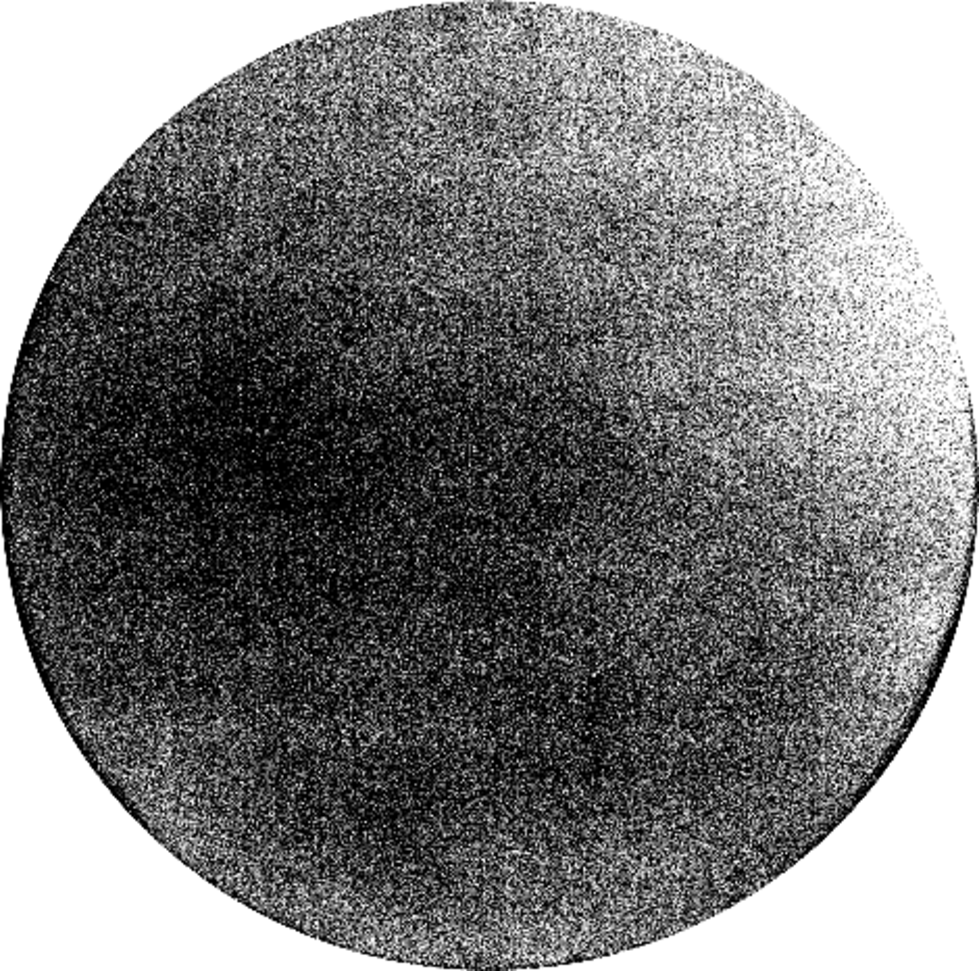
\includegraphics[width=0.5\textwidth,height=0.5\textwidth]{figs/auswertung/plasmaglw/beispieldipolglow.pdf}
%							\end{subfigure}
%							\caption{Ausschnitt aus zwei Bildern der oberen Kamera 'grün' bei einer Dipol-Anregung. Links erliegt die Manipulation. Rechts tragen zwei der vier Segmente, welche zusammengelegt wurden, ein Extremum.}
%						\end{figure}

\newpage

      \subsection*{Fazit}

          Die Analyse des Plasma-Glow in der näheren Umgebung der Manipulations-Elektrode hat Aufschlüsse über die Veränderungen in der Randschicht ergeben. Insbesondere für eine niedrigere Höhe, in welcher später der Yukawa-Ball eingefangen wird, konnten interessante Beobachtungen gemacht werden. Insgesamt hat die Untersuchung einen Einblick dahin gehend ermöglicht, welche Effekte der Anregung und dem Einfang des Clusters zu Grunde liegen. Des Weiteren konnten bereits mögliche Fehlerquellen späterer Messungen erfasst werden.

    \newpage

  \section{Elektrische Manipulation}\label{sec:manip}

    In diesem Abschnitt werden die Messergebnisse der Beobachtungen der unterschiedlichen Manipulationen eines finiten Yukawa-Clusters präsentiert. Dabei wird zuerst auf die Analyse bezüglich der Normalmoden nach Kapitel \ref{subsub:moden} eingegangen. Dem schließt sich entsprechend die Fluidmoden-Betrachtung an. Differenziert wird zusätzlich zwischen den Anregungen mit einer 4- bzw. 6-segmentigen Ring-Elektrode. Die Auswertung der erhaltenen Daten erfolgt mit Rückblick auf die Ergebnisse des vorherigen Abschnitts, da in diesem essentielle Informationen über die Manipulationen mittels der Ring-Elektrode erlangt wurden.

    \subsection{Normalmoden-Analyse}

      Die Auswertungen der Normalmoden-Anteile in der Bewegung des Clusters erfolgt über die Betrachtung der spektralen Leistungsdichte $S\ix{p}\left(\omega\right)$. Die daraus ermittelten Eigenmoden, in welchen verstärkt Energie enthalten ist, werden daraufhin einzeln betrachtet und analysiert.\\
      Bei den gemachten Messungen lag der Argon-Gasdruck zwischen $\unit[6,42-10]{Pa}$. Die eingespeisten Leistungen des rf-Generatos lagen, für die Quadrupol-Anregung, bei $\unit[0,5]{W}$ und, in den Versuchen mit der 6-Segment-Elektrode, bei $\unit[1,4]{W}$. Alle drei Kameras nahmen mit einer Auflösung von $\unit[1280]{px}\times\unit[1024]{px}$ bei 100 \tilt{fps} auf. Die Blenden-Öffnungszeit, dass heißt wie lange Licht auf den \tilt{CCD}-Chip treffen kann, betrug $\unit[8]{ms}$. Kamera 'rot' und 'gelb' nahmen jeweils durch $\unit[60]{mm}$, 'gruen' durch ein $\unit[150]{mm}$ Objektiv auf. Jede Messreihe entsprach 10000 Bildern, was bei der gegebenen Frequenz $\unit[100]{s}$ gleich kam.

        \begin{figure}[!h]
          \centering
          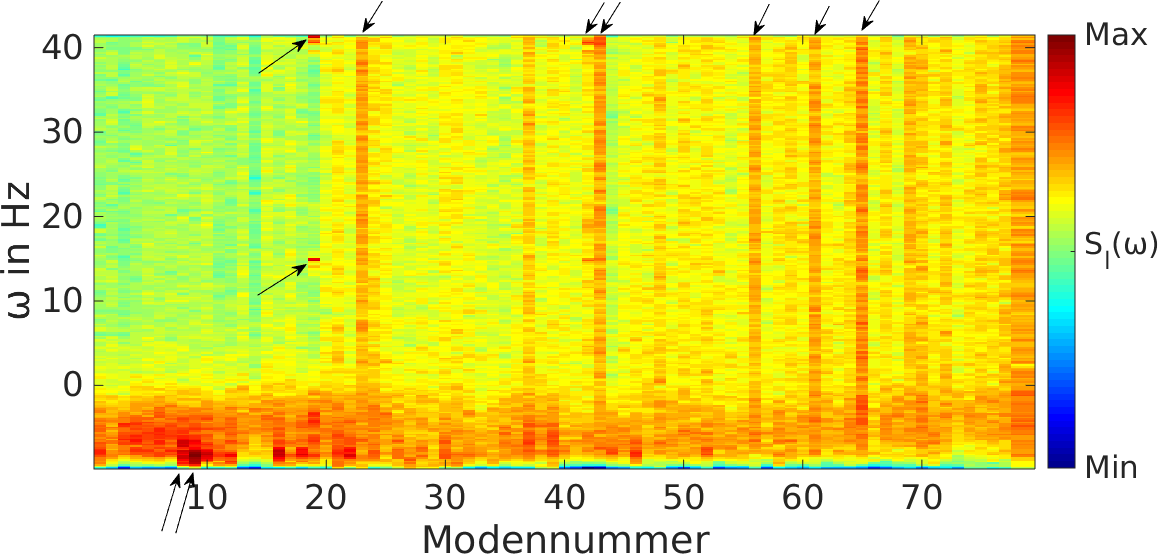
\includegraphics[width=\textwidth]{figs/auswertung/manipulation/ersteungestpowerdens.png}
          \caption{Spektrale Energiedichte $S\ix{p}\left(\omega\right)$ für einen ungestörten Cluster von $N=26$ Teilchen. Die besonders angeregten Moden sind mit Pfeilen und den Nummern markiert.}\label{img:powerdensersteungest}
        \end{figure}

\vspace{-0.4cm}

        \subsection*{Ring-Elektrode mit 4 Segmenten}

          Mit diesem Ring sind vier Messungen zur Quadrupol-Anregung bei unterschiedlichen Frequenzen und einer Teilchenzahl von $N=26$ gemacht worden. Jeweils zwei gegenüberliegende Segmente besaßen dabei das gleiche Potential, wobei insgesamt die beiden sinusoidalen Signale mit einer Amplitude von $U\ix{pp}=\unit[10]{V}$ um eine halbe Periode phasenverschoben waren. Speziell angeregte Moden, die anschließend diskutiert werden, sind in den Energiedichten mit Pfeilen hervorgehoben.

        \begin{figure}[!t]
          \centering
          \begin{subfigure}[t]{0.325\textwidth}
            \centering
            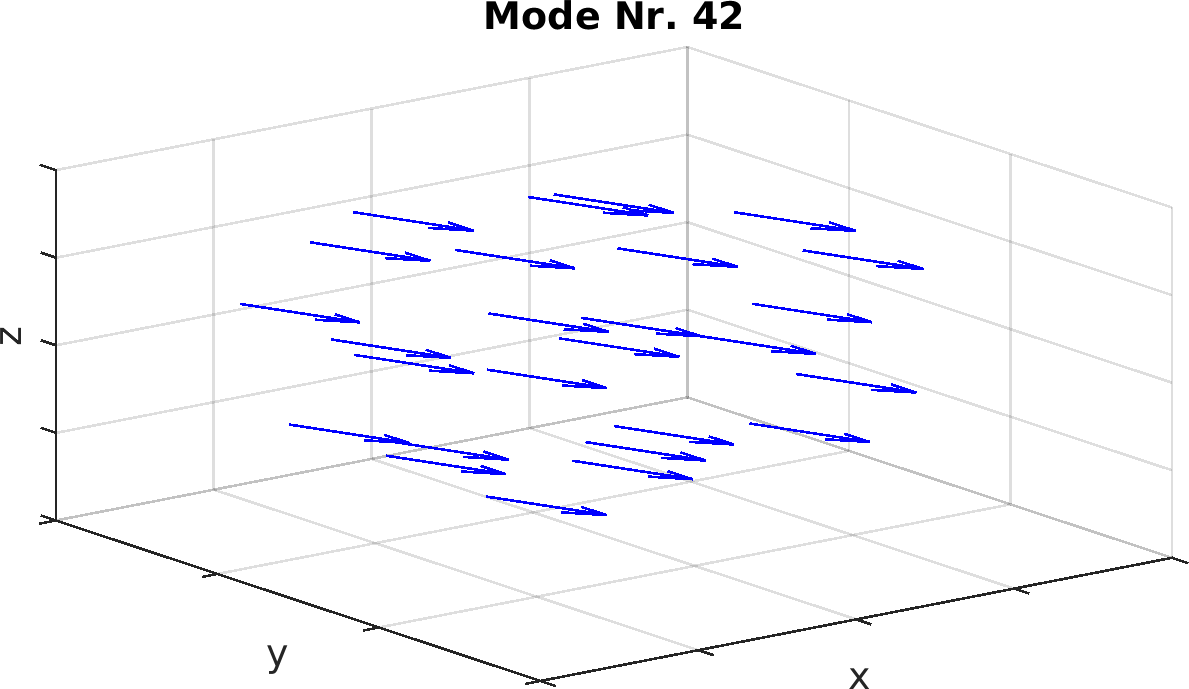
\includegraphics[width=\textwidth,height=0.8\textwidth]{figs/auswertung/manipulation/erstensungestModeNr42.png}
          \end{subfigure}
          \begin{subfigure}[t]{0.325\textwidth}
            \centering
            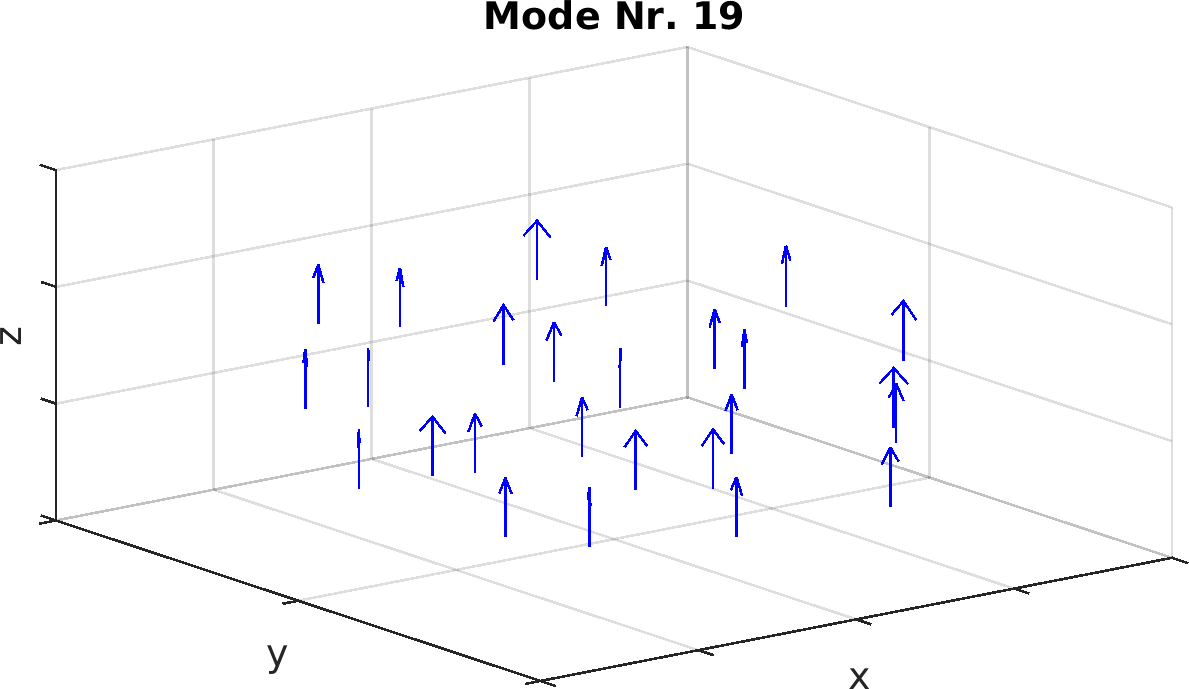
\includegraphics[width=\textwidth,height=0.8\textwidth]{figs/auswertung/manipulation/erstensungestModeNr19.png}
          \end{subfigure}
          \begin{subfigure}[t]{0.325\textwidth}
            \centering
            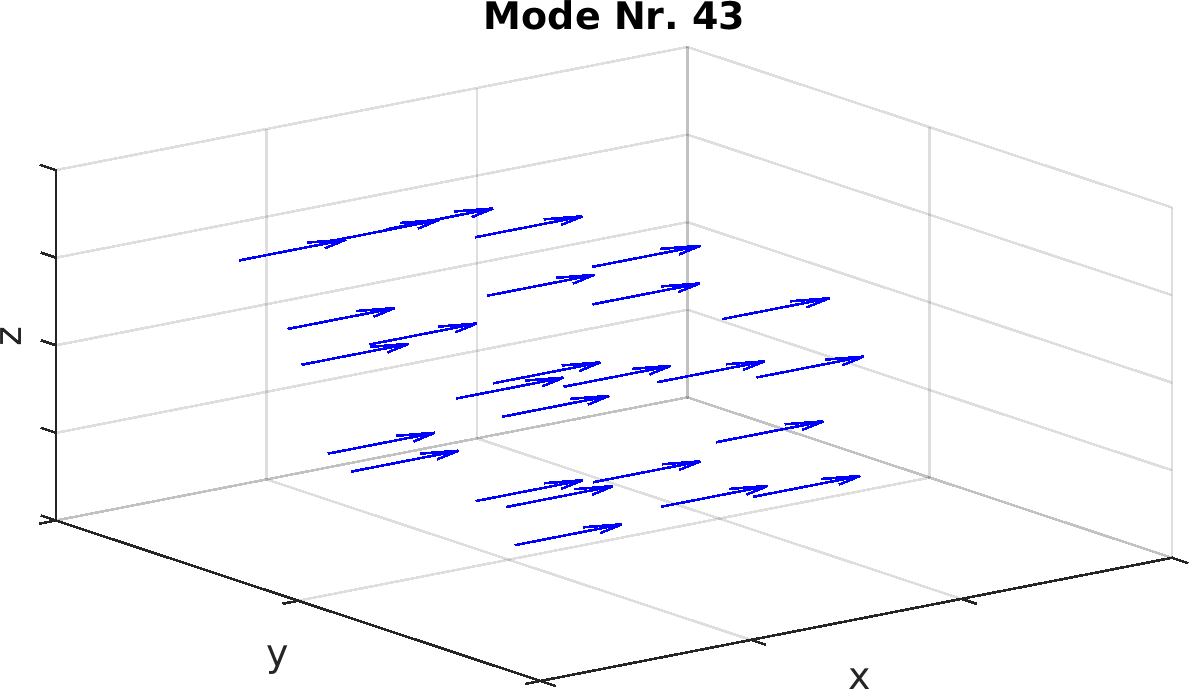
\includegraphics[width=\textwidth,height=0.8\textwidth]{figs/auswertung/manipulation/erstensungestModeNr43.png}
          \end{subfigure}
          \begin{subfigure}[t]{0.325\textwidth}
            \centering
            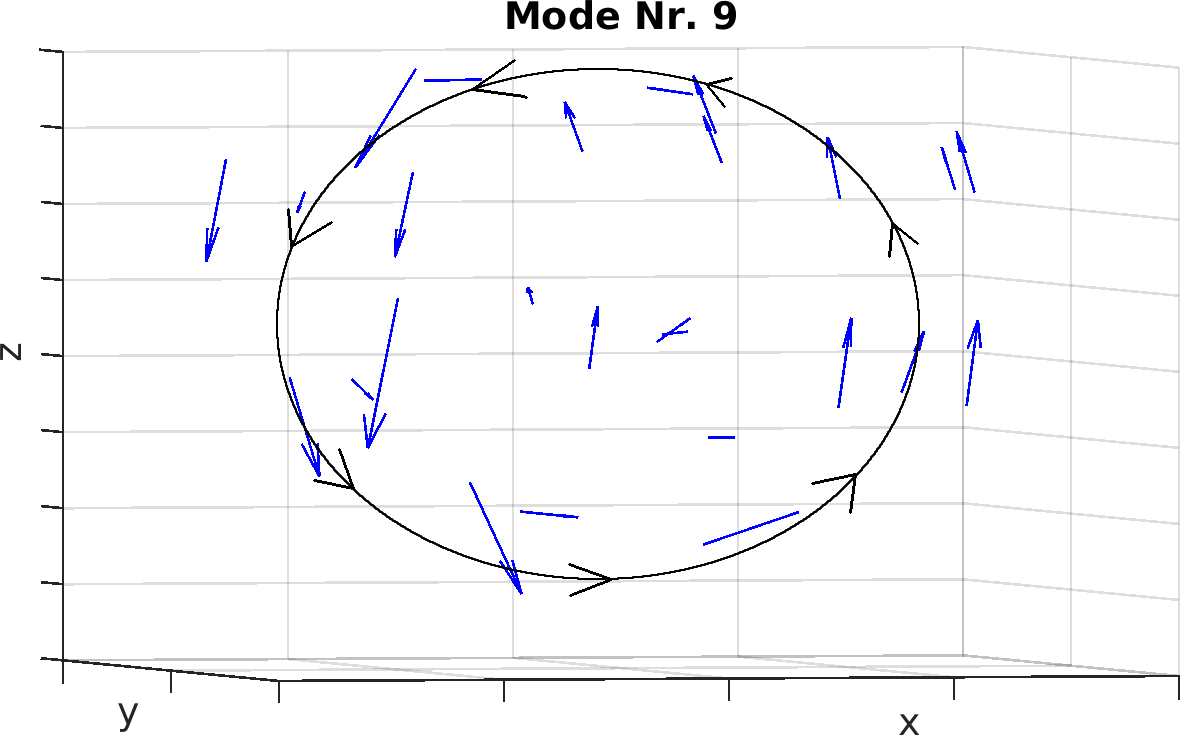
\includegraphics[width=\textwidth,height=0.8\textwidth]{figs/auswertung/manipulation/erstensungestModeNr9.png}
          \end{subfigure}
          \begin{subfigure}[t]{0.325\textwidth}
            \centering
            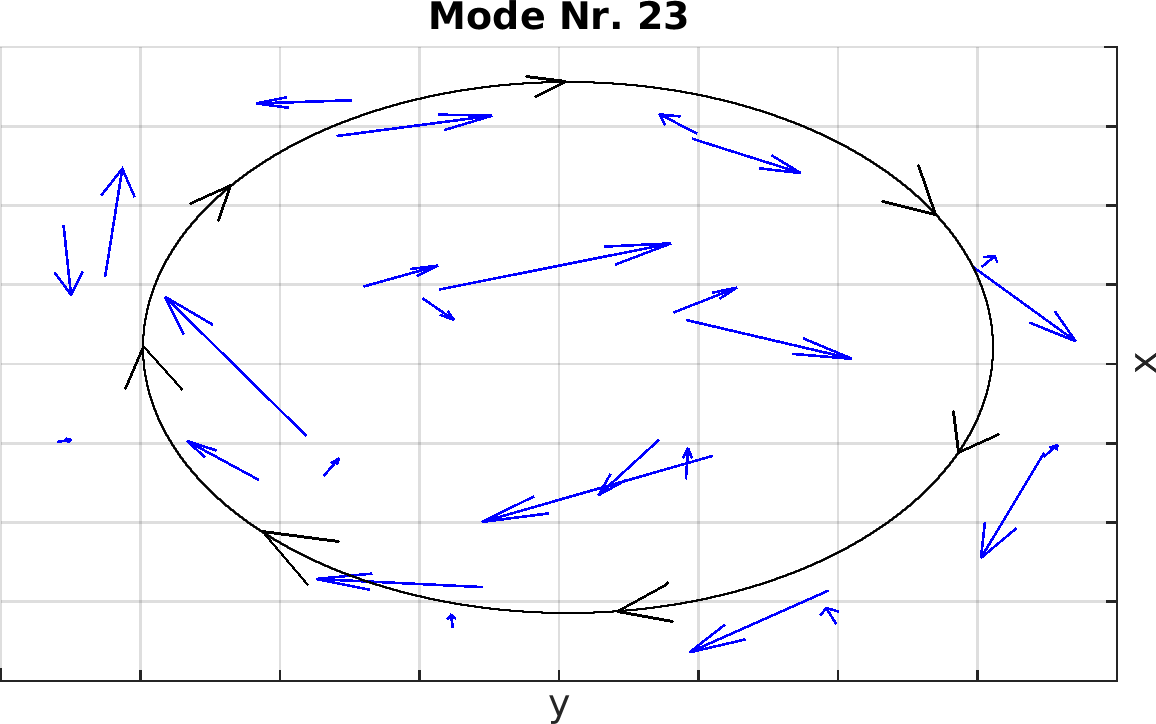
\includegraphics[width=\textwidth,height=0.8\textwidth]{figs/auswertung/manipulation/erstensungestModeNr23.png}
          \end{subfigure}
          \caption{Die Eigenvektoren (blau) der Moden mit den entsprechenden Nummern. In schwarz sind die zu erkennenden Kollektivbewegungen eingezeichnet. Die Auswahl bezieht sich auf die Betrachtungen zu \autoref{img:powerdensersteungest}. Die erste Reihe zeigt die Moden 19, 42, 43. Reihe zwei enthält Nummer 9 und 23.}\label{img:modenersteungest}
        \end{figure}

          Die \autoref{img:powerdensersteungest} zeigt die Dichte für einen ungestörten Cluster von $N=26$ bei den oben genannten Parametern. Mit Pfeilen sind die, entweder für einzelne Frequenzen oder über das gesamte dargestellte Spektrum ($\unit[0-50,5]{Hz}$), energiereichsten Moden hervorgehoben. Im Allgemeinen sind für Frequenzen bis $\unit[10]{Hz}$ alle Moden gut angeregt. Deren Energiegehalt ist dabei in Relationen zu den Moden mit dem größten Anteil an der kollektiven Bewegungen des Clusters dargestellt. Diese Verteilung ist Folge des "`thermischen Chaos"': die zufälligen \tilt{brownschen} Bewegungen der levitierenden Staubpartikel, welche mit bloßem Auge als Zittern wahrnehmbar waren, enthalten viele Moden gleicher Maßen. Die Eigenmoden bzw. -vektoren, welche der Cluster nach Gl.(\ref{eq:ewp}) enthält, sind orthogonal zueinander. Die  thermischen Geschwindigkeitsvektoren $v\ix{th}\left(t\right)$ erfüllen diese Eigenschaft insbesondere nicht, weswegen diese für die Konstruktion der Kollektivbewegung aus vielen verschiedenen Moden zusammengesetzt werden müssen. Speziell die Moden mit der Nummer 35 und höher enthalten mehr Energie. Sie entsprechen chaotischen, voneinander unabhängigen Ein-Teilchen-Translationen.\\
          Interessant sind die markierten Nummern (siehe \autoref{img:modenersteungest}), welche, u.a. über den genannten Bereich hinaus, größere Werte der spektralen Dichte haben. Die Moden 8 und 9 entsprechen Cluster-Rotationen mit einer, zur xy-Ebene parallelen  Drehachse. Sie sind zueinander konjugiert, dh. links- und rechts-drehend (damit orthogonal). Deren korrespondierender Eigenwert liegt, in Übereinstimmung mit Abschnitt \ref{subsub:moden}, bei verschwindend kleinen Frequenzen bzw. bei $\unit[0]{Hz}$. Die Moden 19, 42 und 43 bilden ein, im Sinne eines kartesischen Koordinatensystems, rechtwinkliges Tripel der Clusterbewegung. Jeweils eine dieser Lösungen des Eigenwertproblems zeigt in Richtung einer Achse des Raumes. Des Weiteren stellt Nummer 23 eine Rotation um eine, zur z-Richtung parallelen Achse dar. Die Moden 56, 61 und 65 sind chaotische Bewegungen: die Eigenvektoren haben keine "`besondere"' Anordnung.\\
          Die rechtwinkligen Moden 19, 42 und 43 haben bei der Projektion auf die chaotisch-thermischen Bewegungen der Partikel einen großen Anteil. Die Nummern 8, 9 und 23 kommen durch die Anordnung der Laserstrahlen zustande: die Strahlen sind nicht exakt auf den Mittelpunkt des Clusters fokussiert. Da über deren Querschnitt ein Photonendichte-Gradient existiert, erfahren einige Teile des Yukawa-Balls andere Kräfte durch den unterschiedlichen Strahlungsdruck. Daraus resultiert eine Rotation vom Strahlungsmaximum weg. Da zwei Laser auf den Cluster gerichtet sind, ist es u.U. möglich, dass er um mehrere Achsen rotiert oder seine Gesamtrotation aus verschiedenen zusammengesetzt ist. Daher finden sich mehrere angeregte, dafür zuständige Moden im Spektrum. Für tiefgreifendere Ausführungen zu Laser-induzierten Rotationen siehe \cite{Mulsow13}. Der Kontrast zwischen den Energien niedriger Frequenzen bis $\unit[10]{Hz}$ und darüber resultiert aus den Eigenschaften der \tilt{brownschen} Bewegung.

        \paragraph{Quadrupol-Schwingungen bei 1\,Hz}

            \begin{figure}[!b]
              \centering
              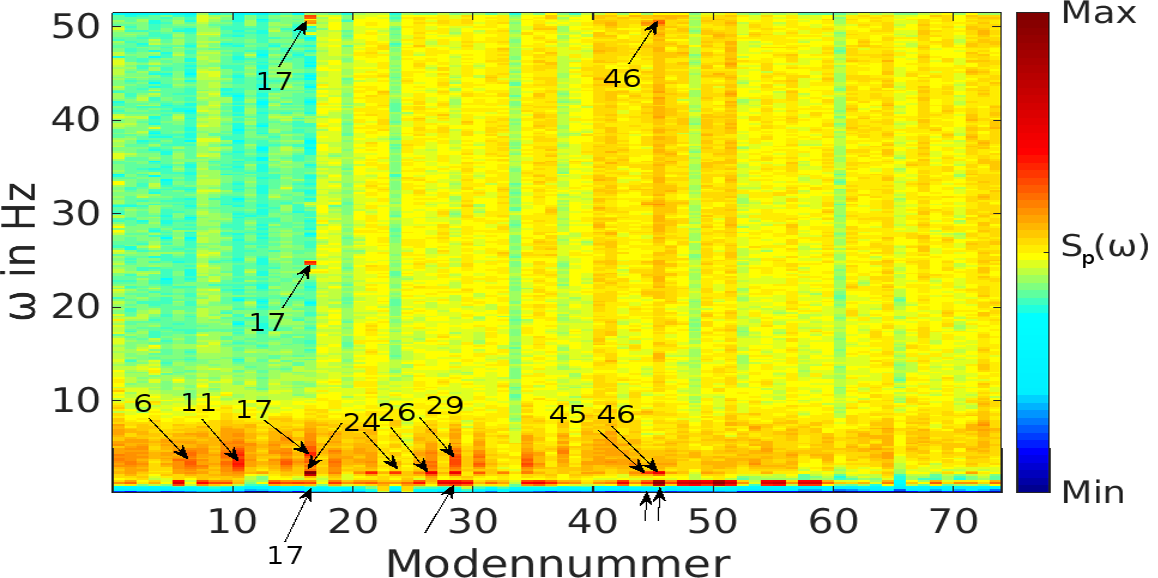
\includegraphics[width=\textwidth]{figs/auswertung/manipulation/quadrupol1Hzpowerdens.png}
              \caption{Spektrale Energiedichte für einen Cluster von $N=26$ Teilchen bei einer Quadrupol-Anregung mit $\unit[1]{Hz}$. Es sind angeregte, höhere Harmonische der Schwingung bei $\unit[2]{Hz}$ zu sehen.}\label{img:powerdensquadrupol1Hz}
            \end{figure}

          In \autoref{img:powerdensquadrupol1Hz} ist die Energiedichte bei Anregung einer Quadrupol-Schwingung bei $\unit[1]{Hz}$ zu sehen. Die Nummern 17, 45 und 46 entsprechen hier den rechtwinkligen Eigenvektoren wie in \autoref{img:modenersteungest}. In diesem Fall enthalten sie im Vergleich zum übrigen Spektrum mehr Energie. Das ist offensichtlich Resultat der Anregung: die Quadrupol-Mode besteht aus Translationen bzw. Cluster-Deformationen auf den Schwigungsachsen. Im speziellen enthält die Nummer 17 eine vergleichbare Energie wie ihre Partner. Jedoch kommt in einer zweidimensionalen Quadrupol-Anregung natürlich keine vertikale Komponente vor. Die Schwingung in z-Richtung ist demnach Folge der Randschichtveränderung in der Mitte des Ringes durch dessen elektrostatische Wechselwirkung mit dem Plasma. Als Referenz sei der vorherige Abschnitt \ref{sub:glowanalys} der Analyse des Plasma-Glow angegeben. Diese vertikale Oszillation enthält besonders viel Energie bei $\unit[2]{Hz}$, da das "`durchschwingen"' der Randschicht gerade mit dem Zweifachen von $\omega$ geschieht.\\
          Sehr scharfe Maxima der Dichte sind bei $\unit[1]{Hz}$ zu sehen. Das zweite, bei einem natürlichen (zwei) Vielfachen der Frequenz auftauchende Maximum entspricht einer höheren Harmonischen der Schwingung. Diese sind gut bei den Moden 24, 26, 29, 45 und 46 zu erkennen. Die Nummern 6, 24 und 29 sind entsprechend Rotationsmoden - siehe \autoref{img:modenquadrupol1Hz}. Anders ist hierbei jedoch, dass es nicht nur eine Drehachse pro Mode gibt, sondern auch beispielsweise gegenläufige Rotationen in einer zusammenkommen (Nummer 6, 26). Ihre Resonanz liegt hierbei jedoch nicht mehr bei $\unit[0]{Hz}$, sonder ist in etwa um eine Anregungsfrequenz nach oben verschoben. Das legt die Vermutung nahe, dass deren Spektrum sich aus den Bewegungen des Quadrupols zusammensetzt und nicht auf Grund der Laser-Anordnung zustande kommt. Neu ist die \tilt{breathing}-Mode 24: sie entspricht einer Ausdehnung des Yukawa-Balls in der Ebene des Quadrupols (parallele zur xy-Ebene). Diese ist schwächer angeregt, da, während der Schwingung auf einer der beiden Achsen dieser Anregung, der Cluster nur minimal senkrecht dazu gestaucht wird. Die Stauchung hat jedoch, als konjugierte Mode zur Ausdehnung, bei der Projektion auf die Deformation einen großen Anteil an der Bewegung. Die Nummer 11 hat kein scharfes Maximum und enthält nur chaotische Eigenvektor-Anordnungen.

            \begin{figure}[!t]
              \centering
              \begin{subfigure}[t]{0.325\textwidth}
                \centering
                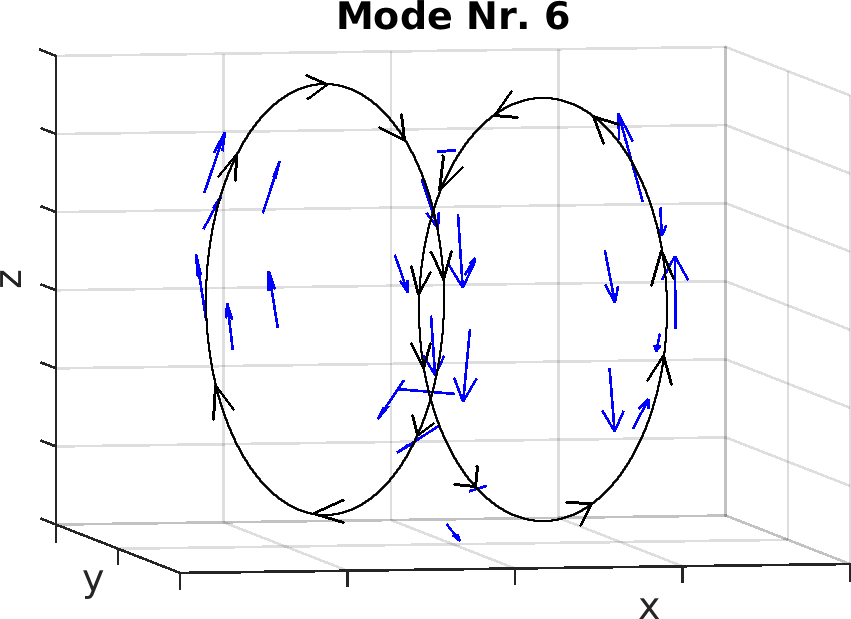
\includegraphics[width=\textwidth,height=0.8\textwidth]{figs/auswertung/manipulation/quadrupol1HzModeNr6.png}
              \end{subfigure}
              \begin{subfigure}[t]{0.325\textwidth}
                \centering
                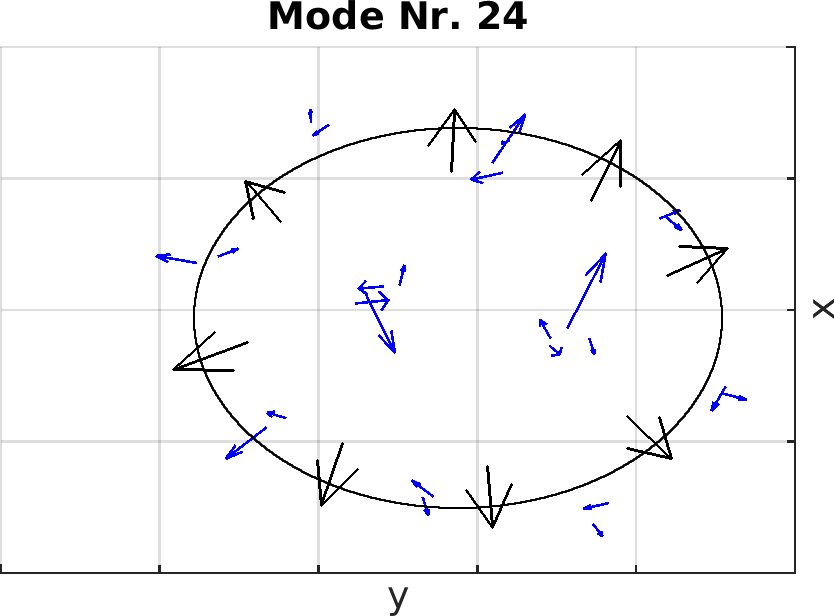
\includegraphics[width=\textwidth,height=0.8\textwidth]{figs/auswertung/manipulation/quadrupol1HzModeNr24.png}
              \end{subfigure}
              \begin{subfigure}[t]{0.325\textwidth}
                \centering
                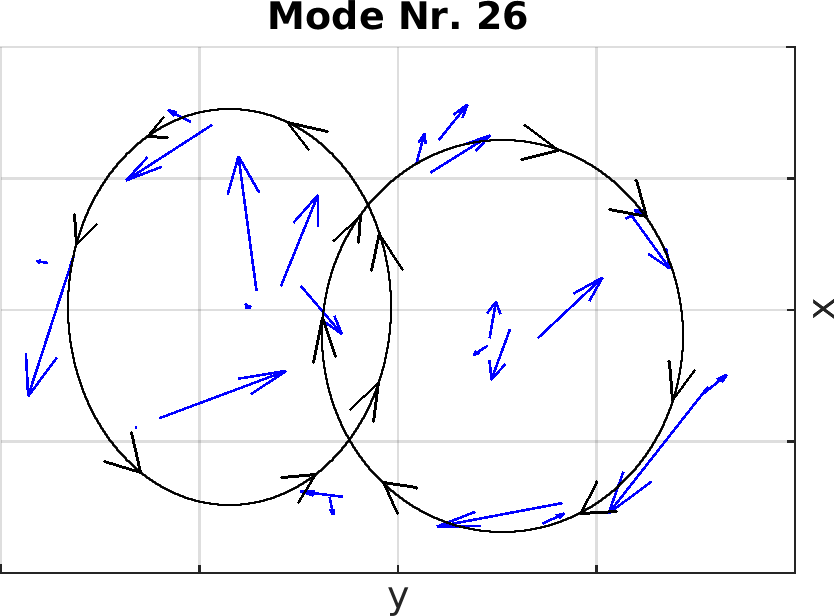
\includegraphics[width=\textwidth,height=0.8\textwidth]{figs/auswertung/manipulation/quadrupol1HzModeNr26.png}
              \end{subfigure}
              \caption{Auszug der, für \autoref{img:powerdensquadrupol1Hz} betrachteten Moden. Insbesondere stehen hier die neuen Rotationen mit mehreren Drehachsen und die \tilt{breathing}-Mode im Fokus.}\label{img:modenquadrupol1Hz}
            \end{figure}


        \paragraph{Quadrupol-Schwingungen bei 3\,Hz}

            \begin{figure}[!b]
              \centering
              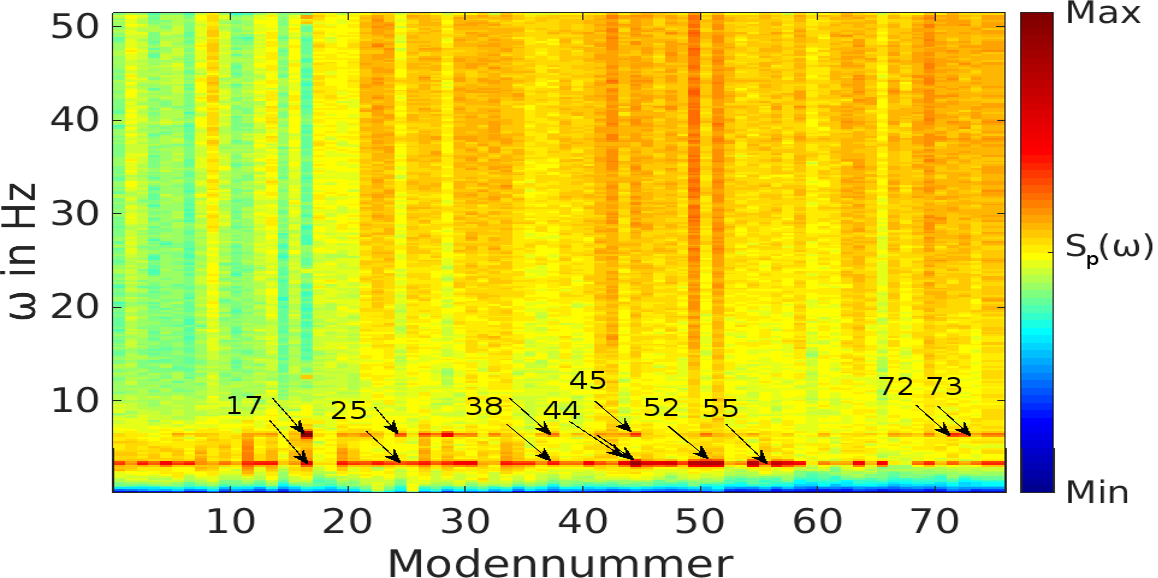
\includegraphics[width=\textwidth]{figs/auswertung/manipulation/quadrupol3Hzpowerdens.png}
              \caption{Spektrale Energiedichte für einen Cluster von $N=26$ Teilchen bei einer Quadrupol-Anregung mit $\unit[3]{Hz}$. Es sind angeregte, höhere Harmonische der Schwingung bei $\unit[6]{Hz}$ zu sehen.}\label{img:powerdensquadrupol3Hz}
            \end{figure}

          In \autoref{img:powerdensquadrupol3Hz} sieht man die Energiedichte für eine Quadrupol-Anregung mit $\unit[3]{Hz}$. Neben der Ähnlichkeit zur Energie-Verteilung \autoref{img:powerdensquadrupol1Hz} fällt auf, dass der Bereich niedriger Frequenzen (bis $\unit[10]{Hz}$) immer weniger eine Rolle spielt: die Dichte ist dort, in Relationen zu den Maxima bei der Anregungsfrequenz, wesentlich geringer. Das heißt, dass die thermische Bewegung innerhalb des Clusters sehr klein gegen die Auslenkungen durch die Anregung ist.\\
          Insbesondere haben die Moden 17, 44 und 45, welche die rechtwinklige Cluster-Translationen sind, gute Extrema bei der ein- und zweifachen Frequenz. Die Nummer 25 ist eine Rotation um eine, zur z-Richtung parallelen Achse. Die Moden 38 und 72 sind beides einatmende \title{breathing}-Moden, das heißt sie stellen Cluster-Ausdehnungen dar. Die Nummer 73 ist die zur 72 konjugierte: eine ausatmende, zusammenziehende \tilt{breathing}-Mode.\\
          Wie bereits besprochen, erfährt der Cluster während der Schwingung entlang einer Achse des Quadrupols eine Deformation auf der anderen. In dieser Richtung wird er gestaucht und verformt sich somit elliptisch.  Die Moden dieser Bewegung sind 52 und 55, welche weiterhin in \autoref{img:modenquadrupol3Hz} gezeigt werden. Diese enthält offensichtlich immer mehr Energie, umso näher die Frequenz an der Eigenfrequenz liegt, weil der Cluster dort die größte Resonanz zeigt. Zu den Eigenfrequenzen schließt sich eine eigene Analyse in Abschnitt \ref{subsec:phasenanal} an. Die Moden der elliptischen Deformation sind deswegen energiereicher: die $\unit[3]{Hz}$ der Anregung liegen in der Nähe von $\omega\ix{0}$. Dies wird ebenso durch den verstärkten Kontrast zu den restlichen Moden bekräftigt. Deren Energiedichte ist, im Vergleich zu den explizit besprochenen sowie der Anregung mit $\unit[1]{Hz}$, viel geringer.

            \begin{figure}[!t]
              \centering
              \begin{subfigure}[t]{0.325\textwidth}
                \centering
                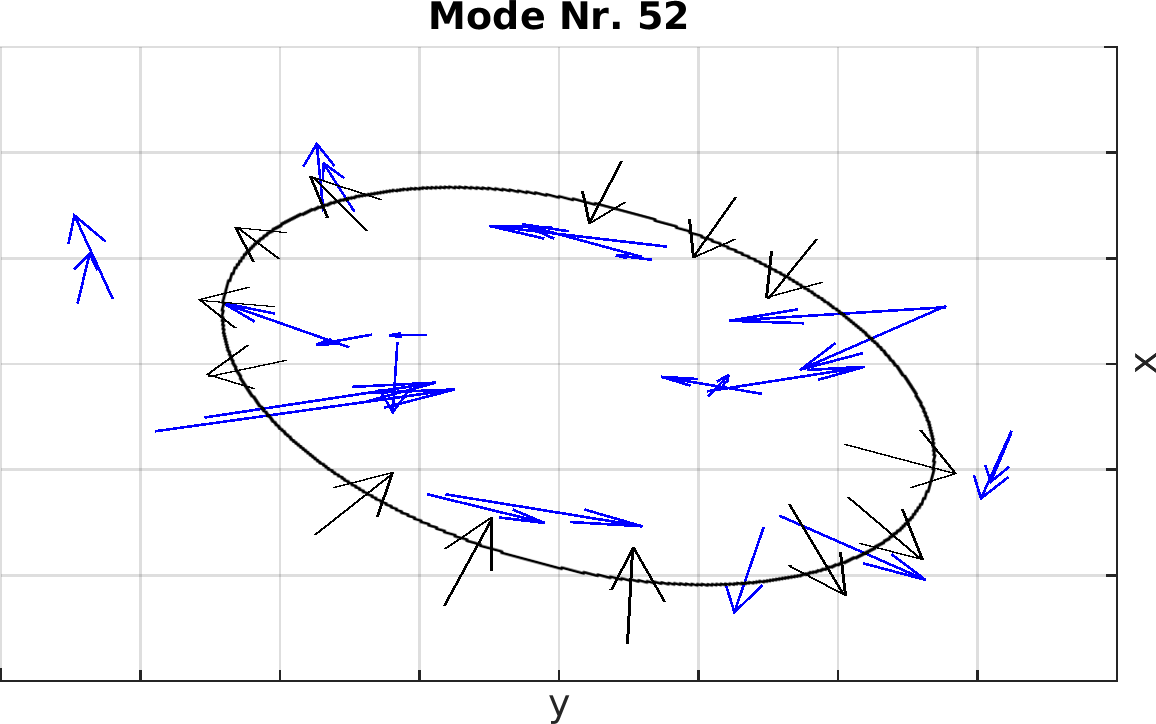
\includegraphics[width=\textwidth,height=0.7\textwidth]{figs/auswertung/manipulation/quadrupol3HzModeNr52.png}
              \end{subfigure}
              \begin{subfigure}[t]{0.325\textwidth}
                \centering
                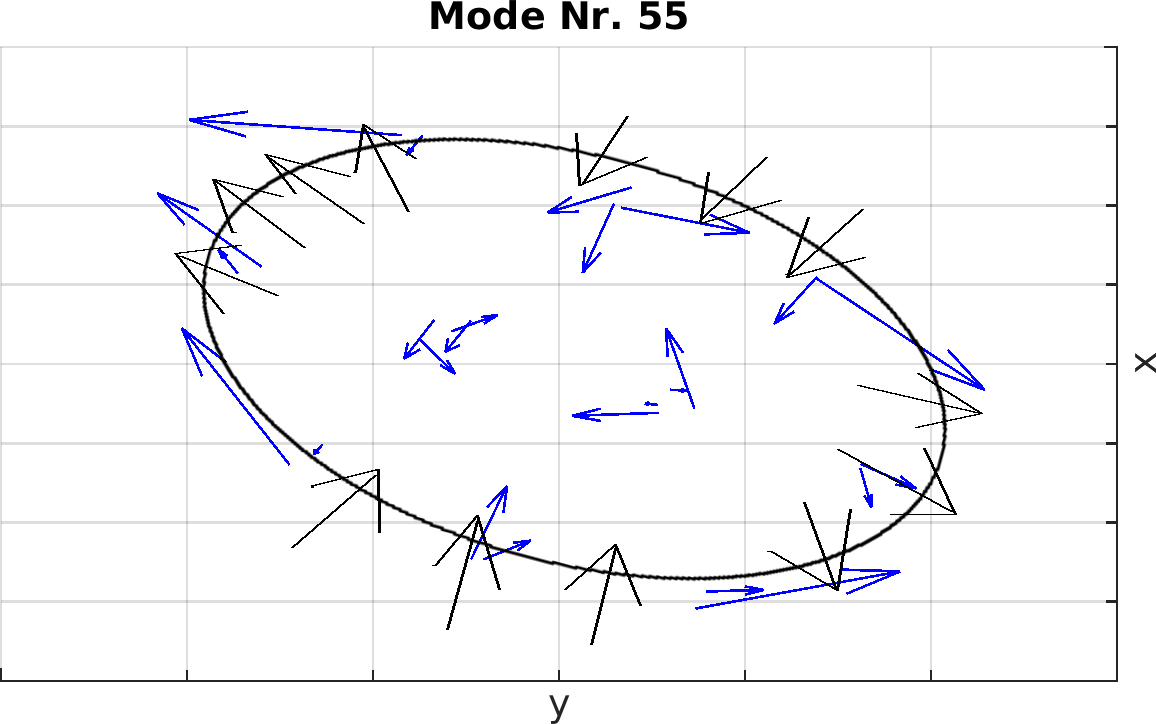
\includegraphics[width=\textwidth,height=0.7\textwidth]{figs/auswertung/manipulation/quadrupol3HzModeNr55.png}
              \end{subfigure}
              \begin{subfigure}[t]{0.325\textwidth}
                \centering
                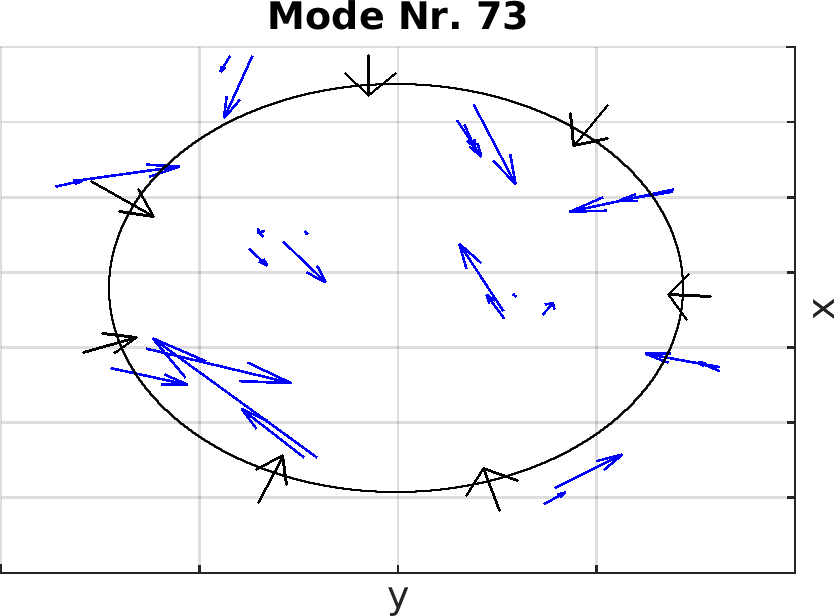
\includegraphics[width=\textwidth,height=0.7\textwidth]{figs/auswertung/manipulation/quadrupol3HzModeNr73.png}
              \end{subfigure}
              \caption{Auswahl der angeregte Moden einer Quadrupol-Schwingung bei $\unit[3]{Hz}$. Neu sind Moden 52 un 55 als elliptische Deformationen während der Auslenkung auf einer Achse.}\label{img:modenquadrupol3Hz}
            \end{figure}

        \paragraph{Quadrupol-Schwingungen mit 5\,Hz}

          Die \autoref{img:powerdensquadrupol5Hz} liefert keine zusätzlichen Informationen über neue, angeregte Moden. Die Nummern 7, 12, 33, 37, 39, 62 und 66 sind chaotische Eigenvektoren. Sie tragen auch hier wiederum signifikant Energie, weil auch aus ihnen alle Cluster-Bewegungen anteilig zusammengesetzt werden können. Analog dazu sind mit 18, 44 und 45 die rechtwinkligen Moden eingetragen. Sie enthalten, der Anregung entsprechend, die meiste Energie. Die Nummern 5, 6 und 32 stellen im Spektrum die Rotationsbewegungen dar.  Hinzu kommen mit 53, 56 und 58 die Quadrupol-Deformationen nach Vorbild von \autoref{img:modenquadrupol3Hz}. Die Nummer 31, 70 und 75 enthalten schließlich ein- bzw. ausatmende (relaxierend, kontrahierend) \tilt{breathing}-Moden.\\
          Die 42 entspricht einer, aus der rechtwinkligen Mode und dessen Konjugiertem zusammengesetzte Bewegung. Der Cluster schwingt dabei entlang einer Achse auf seinen Schwer- bzw. Mittelpunkt zu. Das liefert jedoch keine neuen Informationen über die Kinematik des Systems, da diese Bewegung bereits durch die kollektive Translation in einer Richtung (Nummer 44, 45 und siehe die Moden 42, 43 aus \autoref{img:modenersteungest}) ausgedrückt wird. Sowohl die Resonanz bei der Anregungsfrequenz, als auch der nächsten (bzw. für die Mode 44 übernächsten) Harmonischen sind gut im Spektrum zu sehen.\\
          Insgesamt hat die Dichte im niederfrequenten Bereich, im Vergleich zu \autoref{img:powerdensquadrupol3Hz}, zugenommen, woraus sich schließen lässt, dass der Schritt zu $\unit[5]{Hz}$ die Entfernung zur Resonanzfrequenz $\omega\ix{0}$ vergrößert hat. Ebenso ist auch mehr Energie, als bei einer Anregung von $\unit[3]{Hz}$, in den "`chaotischen"' Moden gespeichert. Das ist als direkte Folge der größeren Differenz zur Eigenfrequenz des Clusters zu verzeichnen. 

            \begin{figure}[!t]
              \centering
              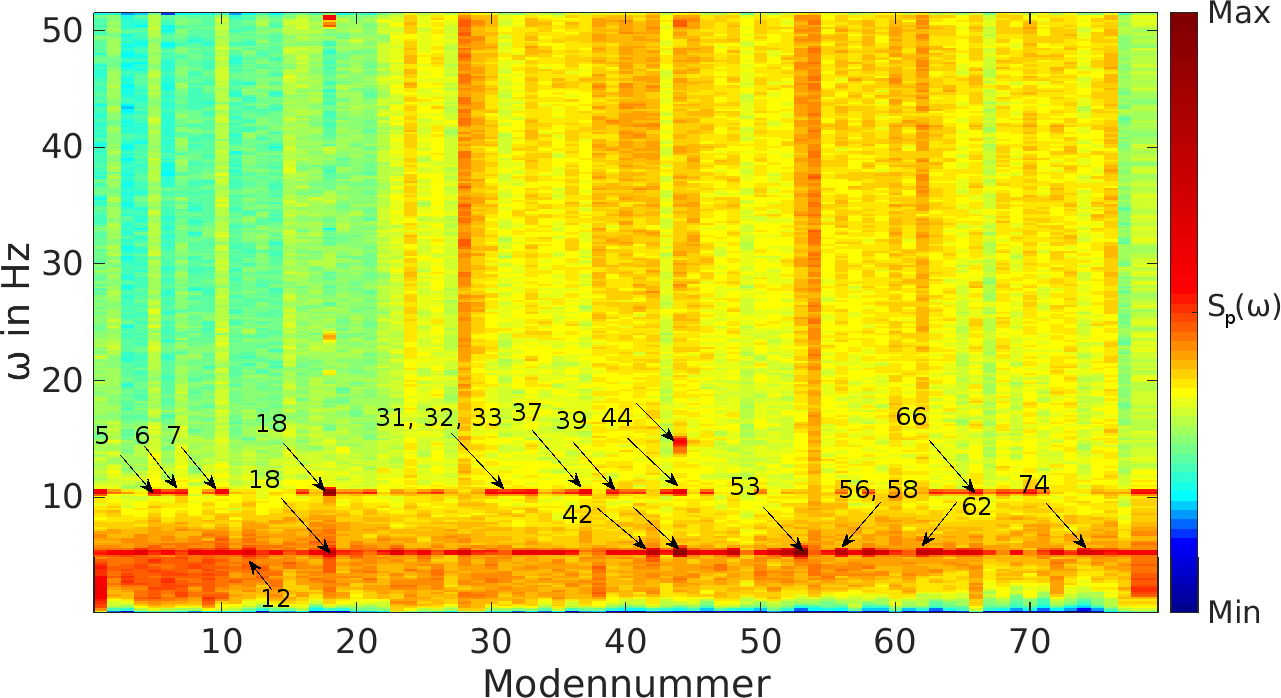
\includegraphics[width=\textwidth]{figs/auswertung/manipulation/quadrupol5Hzpowerdens.png}
              \caption{Spektrale Energiedichte für einen Cluster von $N=26$ Teilchen bei einer Quadrupol-Anregung mit $\unit[5]{Hz}$. Es sind angeregte, höhere Harmonische der Schwingung bei $\unit[10]{Hz}$  und $\unit[15]{Hz}$ zu sehen.}\label{img:powerdensquadrupol5Hz}
            \end{figure}

      \subsection*{Ring-Elektrode mit 6 Segmenten}

%						\begin{figure}[!b]
%							\centering
%							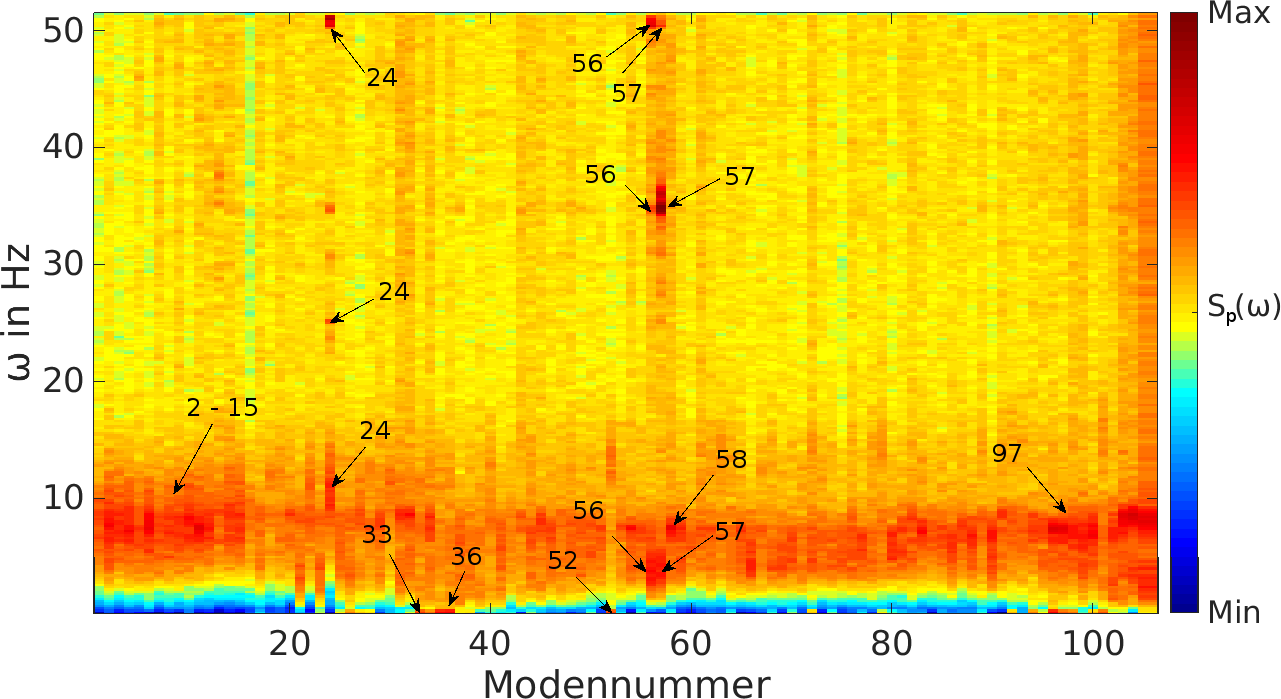
\includegraphics[width=\textwidth]{figs/auswertung/manipulation/zweiteungestpowerdens.png}
%							\caption{Spektrale Energiedichte für einen ungestörten Cluster von $N=31$ Teilchen.}\label{img:powerdenszweiteungest}
%						\end{figure}

        Die Versuche mit der Ring-Elektrode mit 6 Segmenten umfasste Anregungen einer Dipol- und rotieren Dipol-Schwingung. Für den ersten Fall wurden jeweils die Segmente einer Ringhälfte zusammengelegt, sowie mit einer Phasenverschiebung von $\unit[180]{\degree}$ zueinander und Amplitude von $\unit[10]{V}$ \tilt{peak-to-peak} bei verschiedenen Frequenzen versehen. Für die Realisierung eines rotierenden Dipols trugen jeweils 2 gegenüberliegende Segmente das gleiche, sinusoidale Signal. Aufeinander folgende Segmentpaare hatten zueinander eine Phasendifferenz von $\unit[120]{\degree}$, woraus eine Rotationsgeschwindigkeit von einem Ringumfang pro Periode resultierte.

%					Die \autoref{img:powerdenszweiteungest} zeigt die spektrale Energiedichte für einen ungestörten Cluster im 6-Segment-Ring. Analog zu \autoref{img:powerdensersteungest} ist bei niedrigen Frequenzen ein großer Teil der Moden gleichmäßig angeregt. Die Nummern 24, 56 und 57 sind die bekannten rechtwinkligen aus \autoref{img:modenersteungest}. Sie stechen mit ihrem Energie-Dichte-Verlauf, im Vergleich zu den restlichen Moden, heraus. Die Nummern 58, 59, 97-99 und 103 sowie 104 beinhalten chaotisch angeordnete Teilchenbewegungen. Das Rotationsspektrum erstreckt sich über die Moden 2-15, 21, 23, sowie 33-36, wobei die Drehungen um verschiedenste Achsen stattfinden (siehe \autoref{img:modenersteungest} und \autoref{img:modenquadrupol1Hz}). Deren entsprechende Eigenfrequenz liegt, wie zu erwarten, bei $\unit[0]{Hz}$. Schließlich enthalten Nummer 52 und 100-102 Kontraktions- und Ausdehnungs-Moden.

          \paragraph{Dipol-Anregung bei 1\,Hz}

            In \autoref{img:powerdensdipol1Hz} ist die spektrale Energie-Verteilung einer Dipol-Schwingung bei $\unit[1]{Hz}$ zu sehen. Analog zu den vorherigen Anregungen zeigt sich hier im Bereich bis $\unit[10]{Hz}$ eine erhöhte Dichte auf Grund der thermischen Bewegungen. Besonders gut sind jedoch die Maxima bei der Frequenz der Anregung ihr ihrer natürlichen Vielfachen zu erkennen. Für die Dipol-Schwingung scheint es einfacher, ebenso die höheren Harmonischen der Oszillationen anzuregen, da bis auf die Art der Manipulation nichts im Vergleich zu \autoref{img:powerdensquadrupol1Hz} geändert wurde.\\
            Die Mode 27 entspricht der vertikalen Cluster-Translation. In diesem Fall kann dessen Natur sehr gut nachvollzogen werden: im niederfrequenten Bereich hat diese Mode kaum Anteile an der Bewegung des Systems. Jedoch für die Anregungsfrequenz und deren zweifachen bzw. höheren harmonischen sind scharfe Maxima der Dichte zu erkennen. Das ist Ergebnis der Randschichtmanipulation in der Ring-Mitte, aus welcher die vertikale Komponente der Cluster-Schwingung folgt. Außerdem ist in den Moden 57 und 58 besonders viel Energie, relativ zum Mittel aller anderen, enthalten. Diese bilden, zusammen mit 27, das rechtwinklige System aus \autoref{img:modenersteungest}. Alle weiteren, u.U. stärker angeregten Moden sind uninteressant in Hinblick auf die Art der Manipulation.

              \begin{figure}[!t]
                \centering
                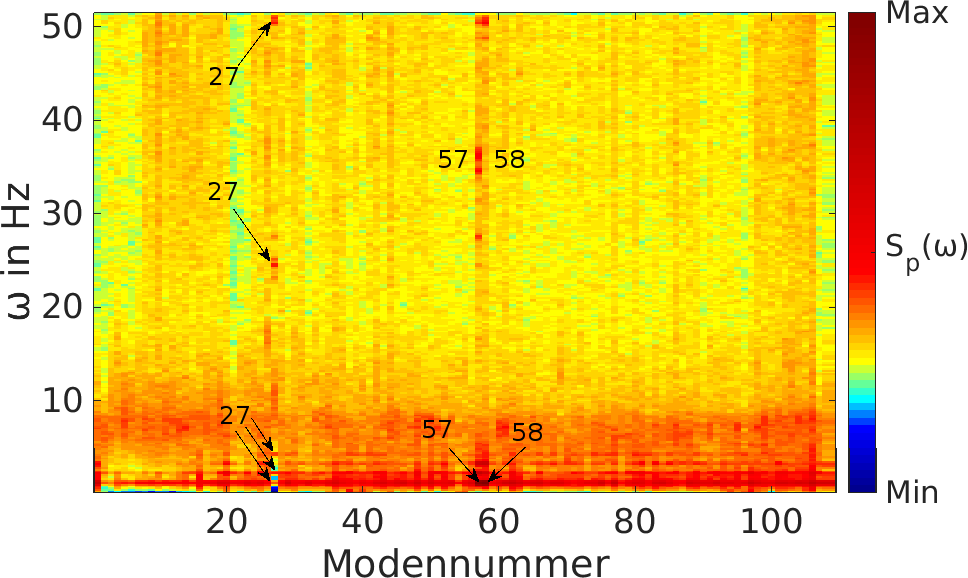
\includegraphics[width=\textwidth,height=0.5\textwidth]{figs/auswertung/manipulation/dipol1Hzpowerdens.png}
                \caption{Spektrale Energiedichte für eine Dipol-Anregung  bei $\unit[1]{Hz}$ eines Cluster von $N=31$ Teilchen.}\label{img:powerdensdipol1Hz}
                \vspace{-0.5cm}
              \end{figure}

          \paragraph{Dipol-Anregung bei 3\,Hz}

            \begin{figure}[!b]
              \centering
              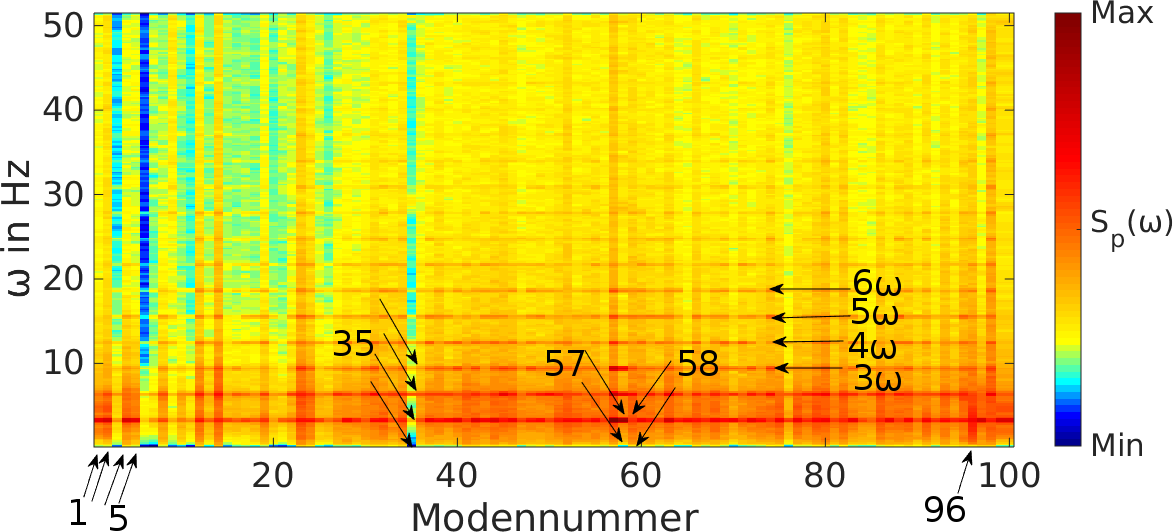
\includegraphics[width=\textwidth]{figs/auswertung/manipulation/dipol3Hzpowerdens.png}
              \caption{Spektrale Energiedichte für eine Dipol-Anregung  bei $\unit[3]{Hz}$ eines Cluster von $N=31$ Teilchen.}\label{img:powerdensdipol3Hz}
            \end{figure}

          Die Aussagen, welche zur Anregung der Dipol-Schwingung mit $\unit[1]{Hz}$ gemacht wurden, treffen für eine mit $\unit[3]{Hz}$, wie sie in \autoref{img:powerdensdipol3Hz} gezeigt ist, noch besser zu. Es können angeregte, höhere Harmonische bis zur sechsfachen Frequenz bei den meisten Moden deutlich erkannt werden. Ebenso gut ist die, auf die Schwingung der Anregung bezogene Mode der vertikalen Oszillation ausgeprägt: über das ganze Spektrum steckt in dieser kaum Energie, außer bei den Vielfachen von $\omega$. Für die korrespondierenden Moden 57 und 58 (kollektive Cluster-Translationen wie zuvor) gilt, das insbesondere bei diesen Frequenzen mehr Energie enthalten ist. Eine einzige Besonderheit zeigt sich jedoch in dem Spektrum dieser Manipulation. Die Nummern 1-5 stellen Verschiebungen einzelner Teilchen dar, während der Reste des Yukawa-Balls ruht. Ein Auszug ist in \autoref{img:modendipol3Hz} zu sehen. Möglicherweise folgt deren erhöhte Energie-Dichte aus ihrer Ähnlichkeit zur Coulomb-Abstoßung der Teilchen und der erzwungenen Bewegungen wie in den Moden 57 und 58.

            \begin{figure}[!t]
              \centering
              \begin{subfigure}[t]{0.325\textwidth}
                \centering
                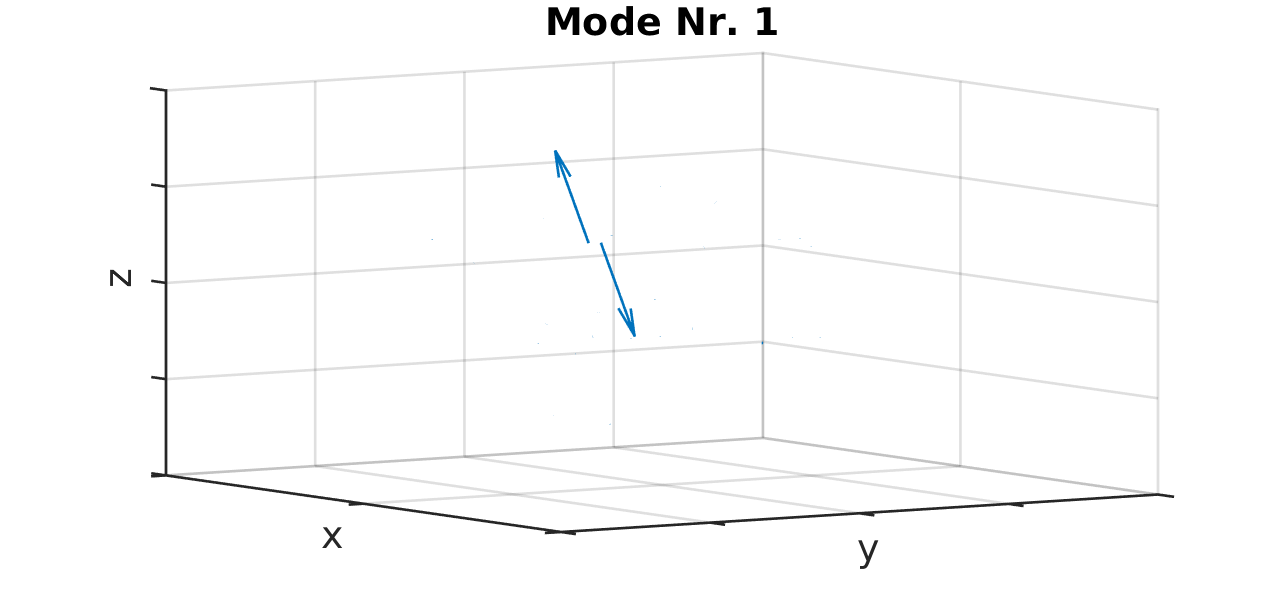
\includegraphics[width=\textwidth,height=0.7\textwidth]{figs/auswertung/manipulation/dipol3HzModeNr1.png}
              \end{subfigure}
              \begin{subfigure}[t]{0.325\textwidth}
                \centering
                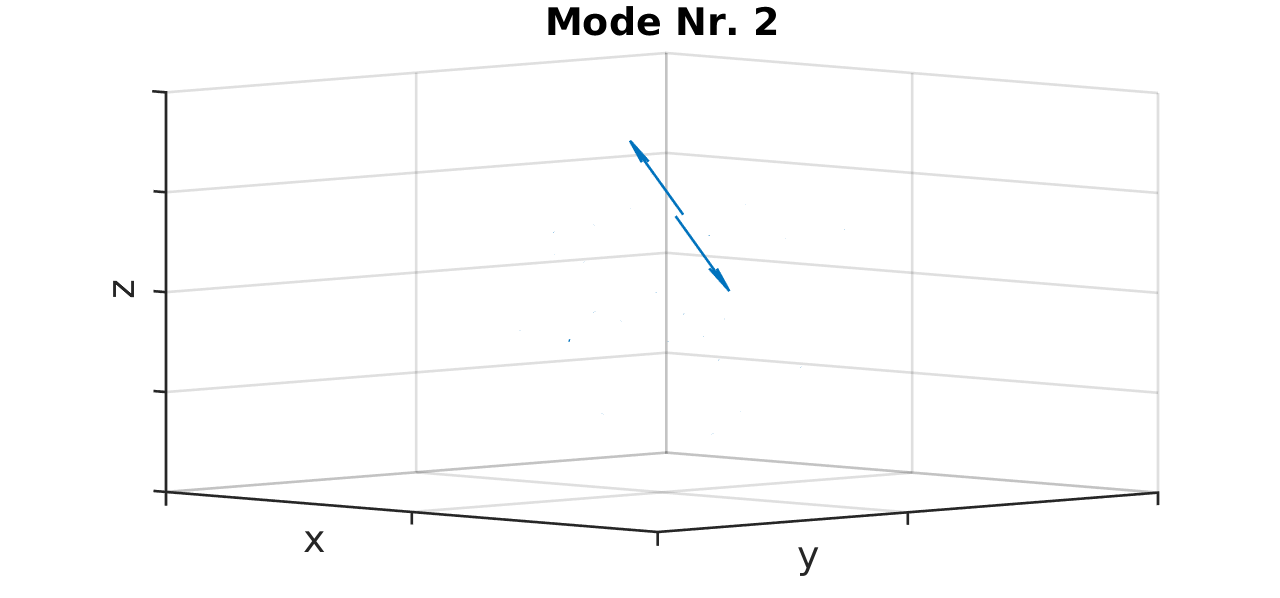
\includegraphics[width=\textwidth,height=0.7\textwidth]{figs/auswertung/manipulation/dipol3HzModeNr2.png}
              \end{subfigure}
              \begin{subfigure}[t]{0.325\textwidth}
                \centering
                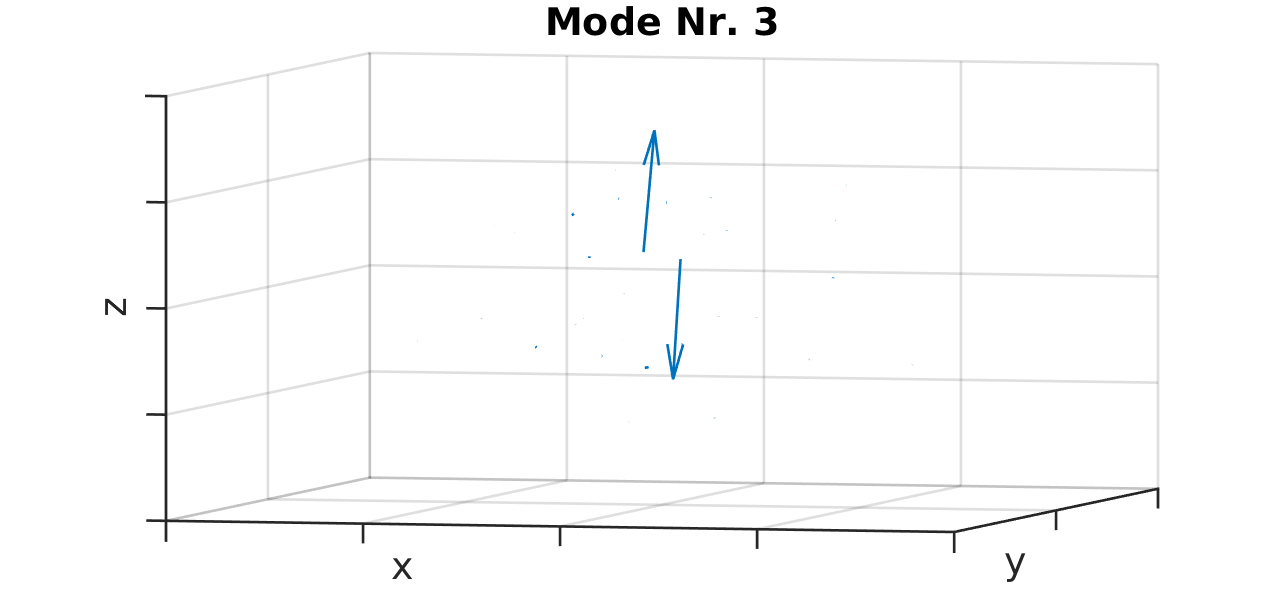
\includegraphics[width=\textwidth,height=0.7\textwidth]{figs/auswertung/manipulation/dipol3HzModeNr3.png}
              \end{subfigure}
              \caption{Auswahl der Moden einer Zwei-Teilchen-Verschiebung bei sonst ruhendem Cluster.}\label{img:modendipol3Hz}
            \end{figure}

          \subsection*{Anregung einer hexagonalen Rotation}

              \begin{figure}[!b]
                \centering
                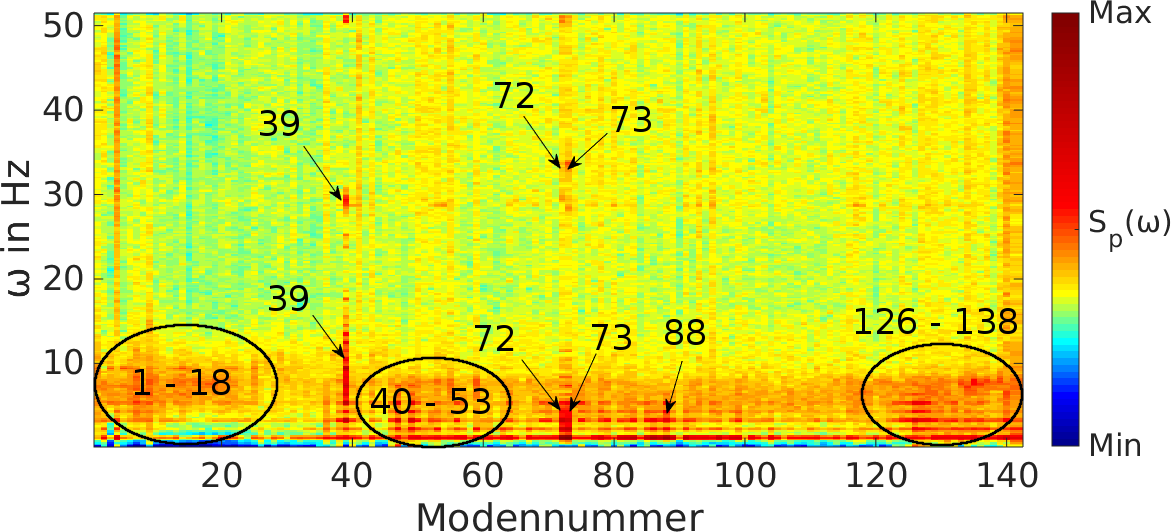
\includegraphics[width=\textwidth]{figs/auswertung/manipulation/rotdipol1Hzpowerdens.png}
                \caption{Spektrale Energiedichte für eine Überlagerung von Rotations- und Deformations-Schwingung bei $\unit[1]{Hz}$.}\label{img:rotdipol1Hzpowerdens}
              \end{figure}

              \begin{figure}[!t]
                \centering
                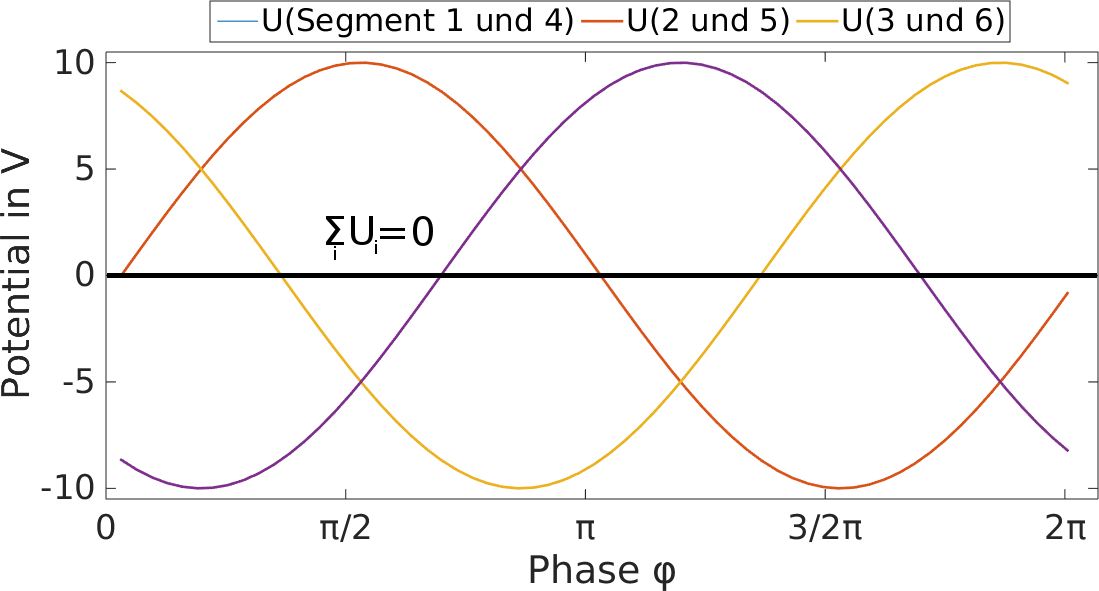
\includegraphics[width=0.8\textwidth]{figs/auswertung/phasen/rotationsverlauf.png}
                \caption{Signalverläufe der verschiedenen Segment bei einer Anregung der hexagonalen Rotation. Der Cluster wird auf einer Achse deformiert und durch die Veränderung des Potentials der darauf folgenden Segmente zur Rotation angeregt. Die Summe der Spannungen ist 0, weswegen die Manipulation um die Gleichgewichtsposition herum stattfindet.}\label{img:signalverlauf}
              \end{figure}

            Nach dem Vorbild der bisherigen Anregungen, wurde mit Hilfe der 6-Segment-Elektrode eine Überlagerung einer Rotation und einer Deformation auf 3 Achsen realisiert. Zwei gegenüberliegende Segmente entsprachen dabei einer Schwingungsrichtung, welche bei der Manipulation um jeweils $\unit[120]{\degree}$ phasenverschoben mit einer Spannung von $\unit[35]{V}$ \tilt{peak-to-peak} und Frequenz von $\unit[1]{Hz}$ betrieben wurden. Die Signalverläufe sind in \autoref{img:signalverlauf} gezeigt. Dadurch vollführt der Cluster, neben der Deformation auf der Achse, zusätzlich eine Torsion im Uhrzeigersinn. Die Messparameter entsprachen dabei denen der bereits besprochenen Versuche. Für einen Cluster aus $N=42$ Teilchen ist in \autoref{img:rotdipol1Hzpowerdens} die spektrale Energie-Dichte dieser Messung dargestellt. Mit Blick auf das Spektrum dieses Experiments kann der Versuch einer gezielten, gleichzeitigen Anregung mehrerer unterschiedlicher Moden als Erfolg betrachtet werden.\\
            Die Moden 39, 72 und 73 sind die rechtwinkligen, kollektiven Cluster-Verschiebungen. Sie sind, wie erwartet, stärker angeregt. Ihre Energie-Dichte liegt sogar, im Vergleich zu den bisherigen Messungen, besonders weit über dem Mittel. Zusätzlich stechen die Bereiche 1-18, 40-53 und 126-138 vor dem "`Hintergrund"' der niederfrequent angeregten, thermischen Bewegungen hervor. Im ersten Fall handelt es sich um eine Kollektion von vertikalen Oszillationen, wobei jedoch im Kontrast zur Mode 39, die Eigenvektoren der Teilchen u.a. nicht vollständig oder sogar anti-parallel zueinander sind. Für sehr niedrige Nummern finden sich sogar die Moden aus \autoref{img:modendipol3Hz} wieder. Diese Anteile sind, analog zu den bis jetzt gemachten Ausführungen, Resultat der Randschicht-Veränderung in der Ring-Mitte.\\
            Der Bereich 40-53 enthält Rotations-Moden. Speziell die Drehung um eine, zur z-Richtung parallele Achse kommt häufiger vor und ist stärker angeregt. Das Ergebnis der phasenverschobenen Dipol-Schwingungen ist demnach ein Impulsübertrag der Staub-Partikel in radialer Richtung auf die nachfolgende Achse zu. Vergleicht man mit den anderen Bereichen, so fällt auf, dass insbesondere hier diskret für die Anregungsfrequenz und dessen Vielfache eine höhere Dichte vorliegt. Im Bereich 126-138 finden sich verschiedenste \tilt{breathing}-Moden, dh. Ausdehnungen und Kontraktionen. Diese treten im Spektrum auf Grund der, über den ganzen Umfang des Clusters stattfindenden Deformationen verstärkt auf. In Kontrast zu einer Quadrupol-Schwingung aus \autoref{img:powerdensquadrupol1Hz} finden, wegen der Drehung der Achsen zueinander, aus- und einatmende Bewegungen in alle Richtungen gleicher Maßen statt.

      \subsection{Phasenaufgelöste Analyse}\label{subsec:phasenanal}

        Nach dem Vorbild der Methode aus Abschnitt \ref{sec:phasen} und den Grundlagen in \ref{subsub:moden} fanden phasenaufgelöste Messungen der Fluidmoden zur Dipol- und hexagonaler Rotations-Schwingung statt. Im Spektrum zwischen $\unit[1,6-6,5]{Hz}$ und bei einer Spannung von $\unit[35]{V}$ \tilt{peak-to-peak} wurden, in Schritten von $\unit[0,1]{Hz}$, für 50 Schwingungen jeweils 4 Bilder gemacht. Da die Aufnahme bei bestimmten Phasen der Anregung erfolgte, knn daraus die Bestimmung der Resonanz vorgenommen werden. Es ergibt sich die Schwingungsantwort des Clusters für einen niederfrequenten Bereich.

        \paragraph{Dipol-Schwingung}
        
          \begin{figure}[!t]
            \centering
            \begin{subfigure}{0.49\textwidth}
              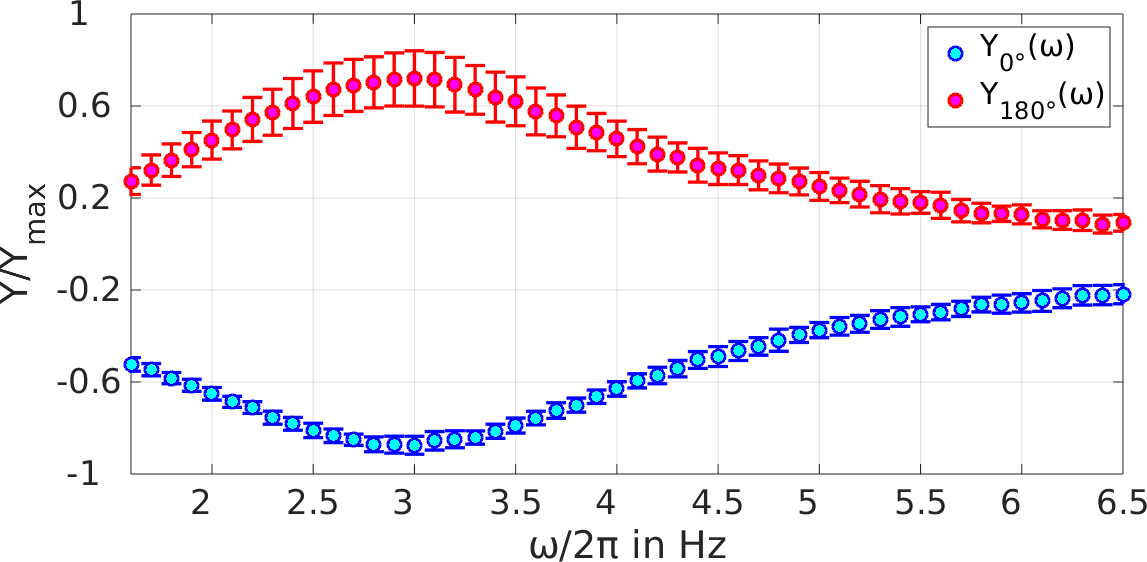
\includegraphics[width=\textwidth,height=0.6\textwidth]{figs/auswertung/phasen/dipolamplitude0180.png}
              \caption{}
            \end{subfigure}
            \begin{subfigure}{0.49\textwidth}
              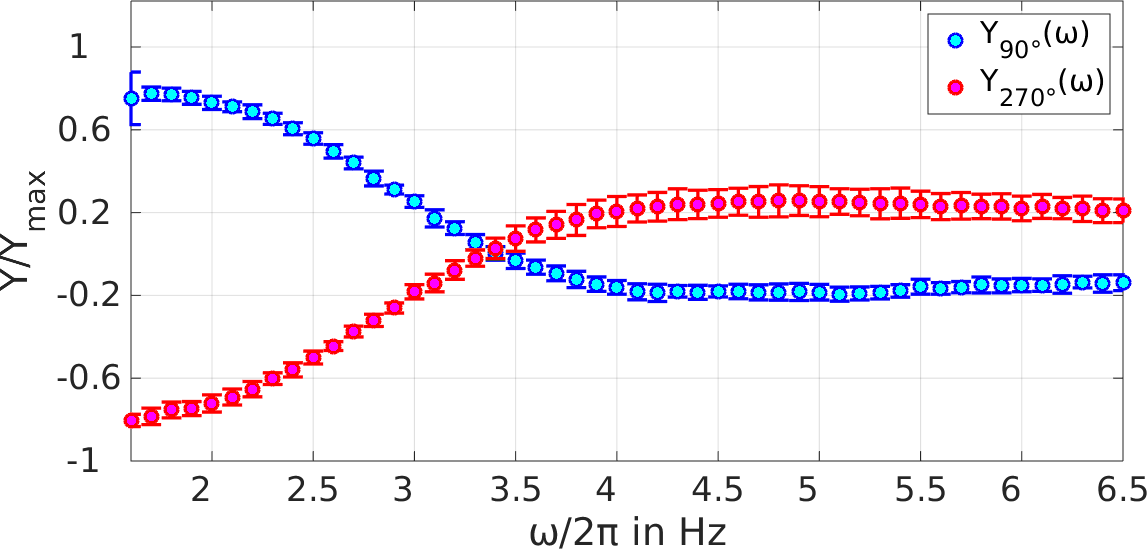
\includegraphics[width=\textwidth,height=0.6\textwidth]{figs/auswertung/phasen/dipolamplitude90270.png}
              \caption{}
            \end{subfigure}
            \caption{Amplituden mit Fehlerbalken entlang der Richtung der Schwingung (\fett{(a)}) und orthogonal dazu (\fett{(b)}). Beide Verläufe nähern sich dem gleichen Bild mit größeren Frequenzen an.}\label{img:dipolamplituden}
          \end{figure}

          \begin{figure}[!b]
            \centering
            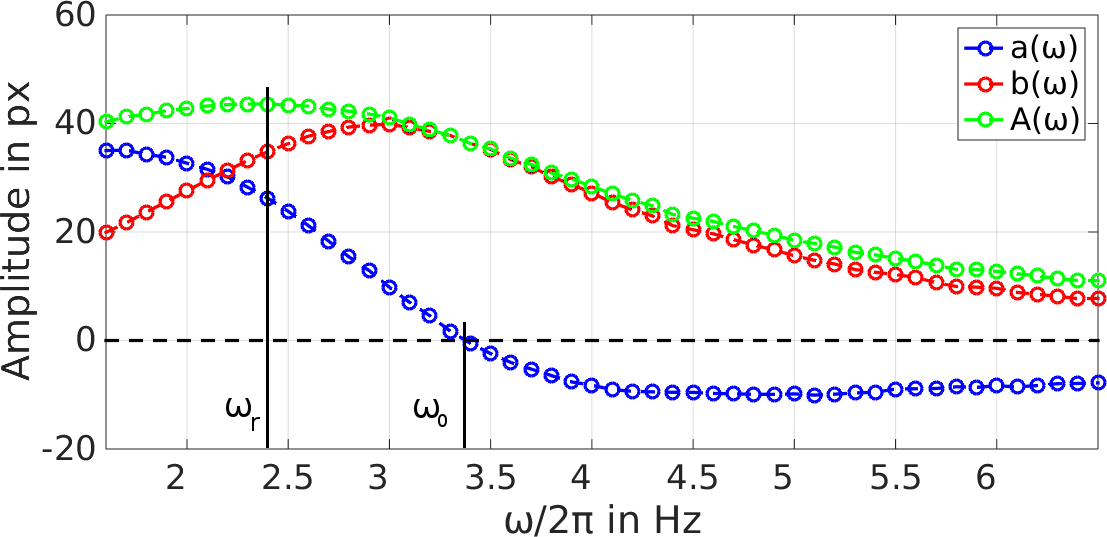
\includegraphics[width=0.8\textwidth,height=0.4\textwidth]{figs/auswertung/phasen/dipolphasenaufg.png}
            \caption{Zusammengeführte Daten der Schwingungsrichtungen. Nach \autoref{img:amplitud} sind $\omega\ix{r}$ und $\omega\ix{0}$ eingezeichnet.}\label{img:resonanzundomega}
          \end{figure}

          Bestimmt man die (feste) Schwingungsachse, so lassen sich für $a\left(\omega\right)$ und $b\left(\omega\right)$ aus den Zuständen bei den Phasen $0\degree$, $90\degree$, $180\degree$ und $270\degree$ diskrete Werte bestimmen. Zuerst werden jedoch die Amplituden der Cluster-Bewegungen auf der Dipol-Achse und senkrecht zu dieser ermittelt. Das Ergebnis ist in \autoref{img:dipolamplituden} gezeigt. Entlang der Anregung, also um die Richtung von $\unit[0]{\degree}$ und $\unit[180]{\degree}$, sind kurz vor $\unit[3]{Hz}$ Extrema zu finden. Bei dieser Frequenz befindet sich demnach die Resonanz, da für eine Schwingung mit $\omega\ix{r}$ die Amplituden divergieren bzw., im realen Fall, maximal werden. Hier sind die Auslenkungen auf ihr Maximum normiert worden. Die Amplituden der Oszillationen senkrecht zur Dipol-Achse verschwinden für eine Anregung mit etwa $\unit[3,5]{Hz}$. Hier liegt die Eigenfrequenz des Clusters. Der Unterschied zwischen beiden liegt in der nicht-verschwindenden Dämpfung der Schwingung und der, nicht ganz vollständigen Beschreibung des Systems im Eigenwertproblem aus \autoref{eq:ewp}. Die Resonanzfrequenz, welche auf Grund des Faktors $\gamma$ immer echt kleiner als $\omega\ix{0}$ ist, zeigt deswegen die stärkste Schwingungsantwort an. Bei einer Anregung mit der Eigenfrequenz hingegen oszilliert der Cluster nur mit der Manipulation und es gehen keine Anteile verloren. Für größere Frequenzen zeigt sich in beiden Richtungen das gleiche Bild: das System kann der Anregung nicht mehr richtig folgen und führt nur noch ungerichtete, chaotische Bewegungen aus.\\
          Die zusammengeführten Daten werden in \autoref{img:resonanzundomega} dargestellt. Resonanz- und Eigenfrequenz liegen in den erwarteten Bereichen. Somit können die Annahmen aus den vorherigen Abschnitten als bestätigt angenommen werden. Des weiteren erkennt man gut, dass die Antwort des Systems in jeglicher Hinsicht mit höheren Frequenzen immer geringer wird.

        \subsubsection*{Hexagonale Rotations-Anregung}

            \begin{figure}[!t]
              \begin{subfigure}{0.49\textwidth}
                \centering
                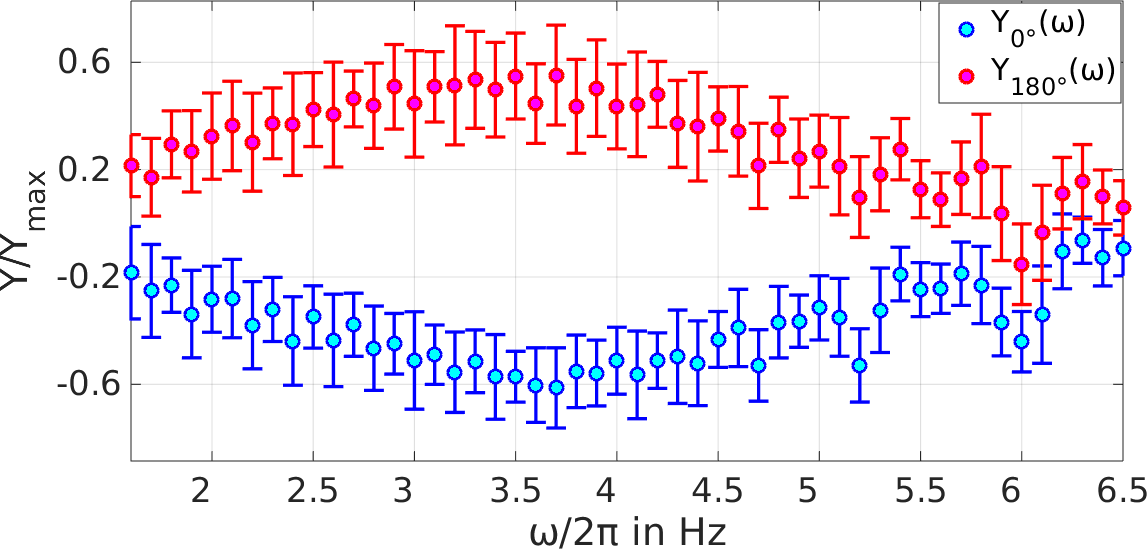
\includegraphics[width=\textwidth,height=0.6\textwidth]{figs/auswertung/phasen/rotamplitude0180.png}
                \caption{}
              \end{subfigure}
              \begin{subfigure}{0.49\textwidth}
                \centering
                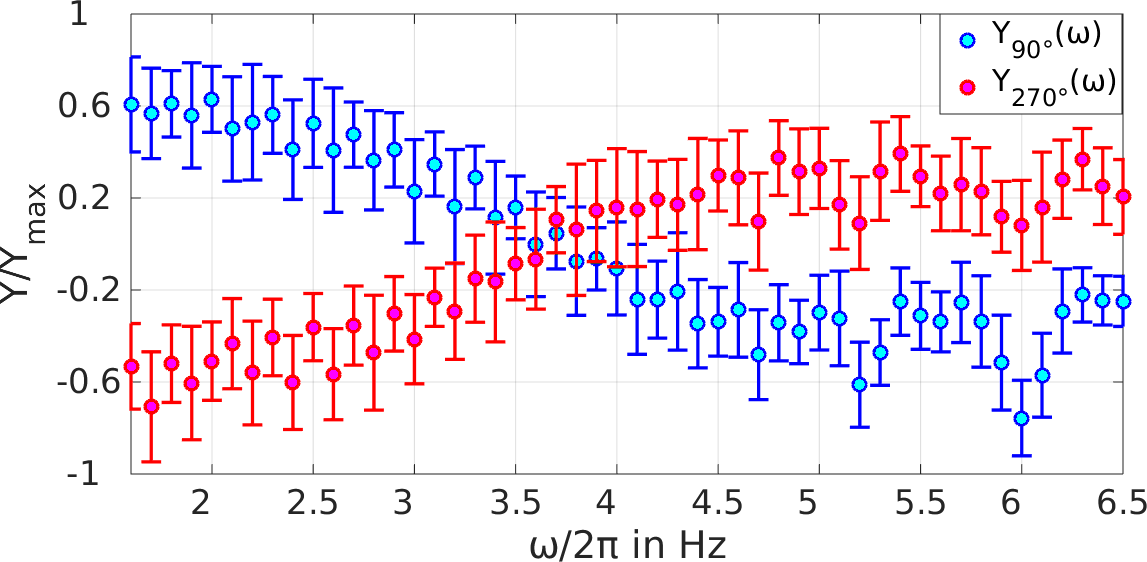
\includegraphics[width=\textwidth,height=0.6\textwidth]{figs/auswertung/phasen/rotamplitude90270.png}
                \caption{}
              \end{subfigure}
              \caption{Amplituden mit Fehlerbalken für eine feste Achse (in \fett{(a)}) und senkrecht dazu (in \fett{(b)}). Bei $\omega\ix{r}\approx\unit[3,7]{Hz}$ verschwindet die Auslenkung in orthogonaler Richtung zur Anregung.}\label{img:hexarotamp}
              \vspace{-0.5cm}
            \end{figure}

          \begin{figure}[!b]
            \centering
            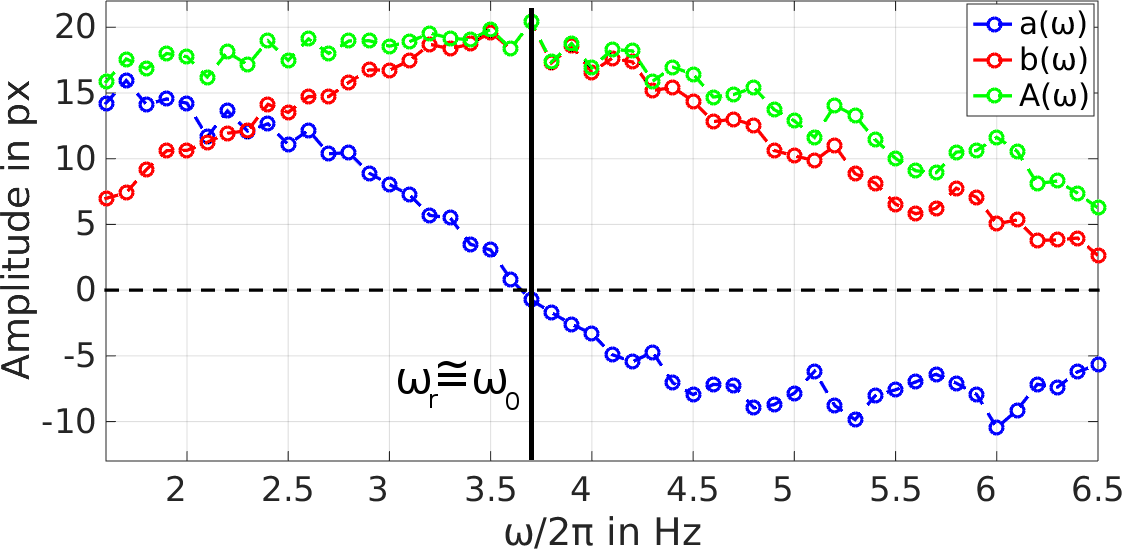
\includegraphics[width=0.8\textwidth,height=0.37\textwidth]{figs/auswertung/phasen/rotphasenaufg.png}
            \caption{Zusammengeführte Daten der Schwingungsrichtungen. Die Frequenzen $\omega\ix{r}$ und $\omega\ix{0}$ fallen in etwa zusammen. Im Vergleich zu \autoref{img:resonanzundomega} sind die Amplituden halb so groß.}\label{img:hexarotphas}
          \end{figure}

          Die Potentiale der einzelnen Signale sind in \autoref{img:signalverlauf} gezeigt. Für die Summe der Spannungen gilt, dass diese zu jedem Zeitpunkt verschwindet. Die Manipulation erfolgt demnach nur um das Gleichgewicht herum und stört den Cluster nicht asymmetrisch. Auch hier kann man eine Analyse bezüglich der Amplituden der Schwingungen vornehmen. Dafür werden die Deformationen des Clusters auf einer festen Achse und senkrecht dazu als Auslenkungen gemessen und in \autoref{img:hexarotamp} dargestellt. Im Unterschied zur Schwerpunktstranslation bei einer Dipol-Schwingung, führt das System nur eine Ausdehnung bzw. Kontraktion in Richtung der drei verschiedenen Achsen aus. Da jedoch gleichzeitig in allen diesen Richtungen eine Manipulation stattfindet, sind die Verhältnisse von Eigen- und Resonanzfrequenz verändert. Zudem verkleinern sich durch das "`ziehen in 2 Richtungen"' auch die Amplituden. Die Größen $\omega\ix{r}$ und $\omega\ix{0}$ fallen bei ca. $\unit[3,7]{Hz}$ zusammen. Bei einer Anregung mit dieser Frequenz ist die Antwort des Clusters maximal und scharf ausgeprägt. Auslenkungen in andere Richtungen erfolgen höchstens durch thermische Oszillationen, nicht jedoch als Folge der Manipulation. Die Resonanzfrequenz liegt so nahe an der Eigenfrequenz, weil zusätzlich zum eigentlichen Einfang eine Kraft durch die Spannungen auf den übrigen Segmenten folgt. Dadurch ist die Schwingung in einer Richtung begünstigt, was zu einer Verminderung des Einflusses der Reibung mit $\gamma$ führt. Die Abbildung \autoref{img:hexarotphas} bestätigt die Beobachtungen.

      \subsection{Gyrations-Trajektorien}\label{sub:gyrat}

          \begin{figure}[!t]
            \begin{subfigure}{0.49\textwidth}
              \centering
              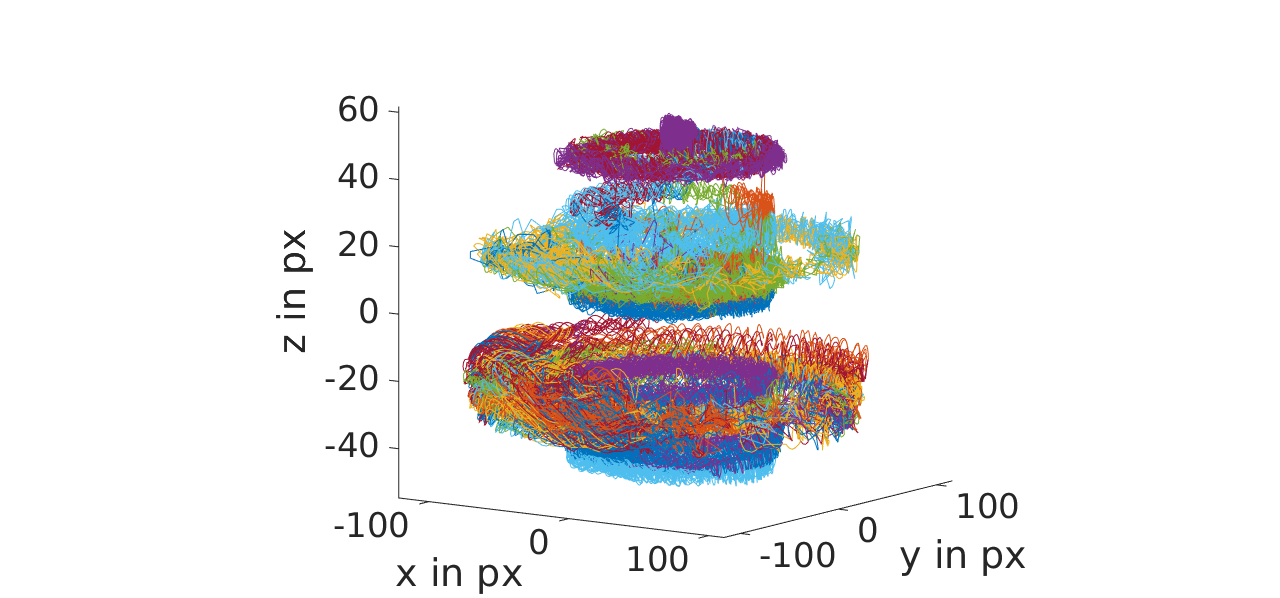
\includegraphics[width=\textwidth,height=0.8\textwidth]{figs/auswertung/trajectoriesrot.png}
              \caption{}\label{img:volltraj}
            \end{subfigure}
            \begin{subfigure}{0.49\textwidth}
              \centering
              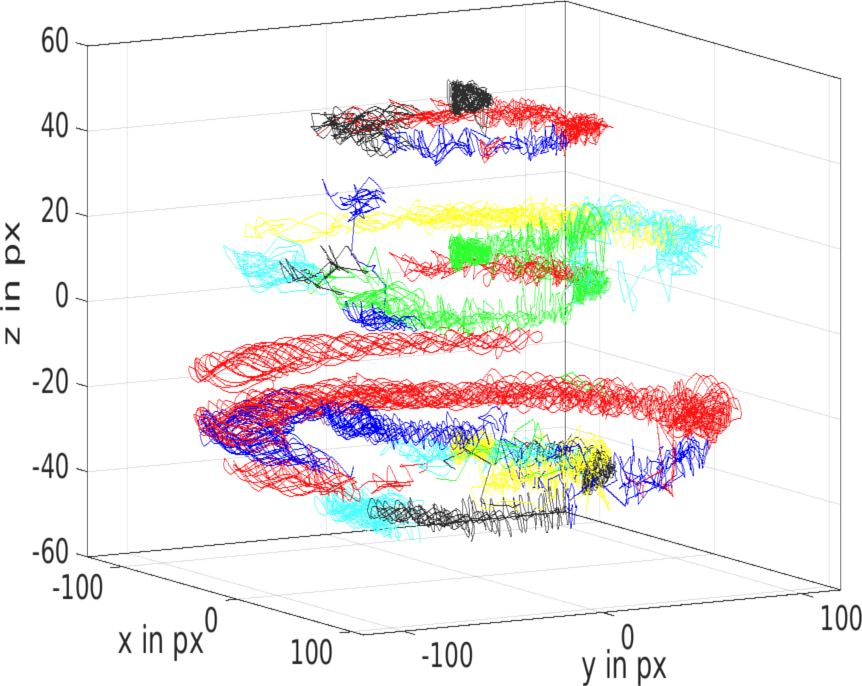
\includegraphics[width=\textwidth,height=0.8\textwidth]{figs/auswertung/trajectoriesrotkurz.png}
              \caption{}\label{img:kurztraj}
            \end{subfigure}
            \caption{Volle Trajektorien eines Clusters von $N=42$ bei hexagonaler Rotations-Anregung über einen Zeitraum von $\unit[100]{s}$ in \fett{(a)}. Unterschiedliche Farben kodieren die Partikel. Verkürzte Teilchen-Bahnen nur für einen Zeitraum von $\unit[10]{s}$ in (\fett{b}).}
          \end{figure}

        Bei der Betrachtung der vollständigen Trajektorien des Clusters, wie sie in \autoref{img:volltraj} und \autoref{img:kurztraj} gezeigt sind, fällt auf, dass die mutmaßliche Rotation durch eine neue Art der Bewegung zu Stande kommt. Die Teilchen "`wandern"' nämlich nicht, so wie es die Anregung hatte vermuten lassen, auf einer Zick-Zack-Bahn über einem Kreis um (Vergleich \autoref{img:trajektorienvergleich}). Vielmehr führen sie eine Gyration parallel zu der kollektiven Cluster-Rotation aus. Auf Grund der ebenso angeregten Randschicht-Verformung in der Ring-Mitte enthalten diese Bewegungen zusätzliche vertikale Komponenten, die letztendlich die Gyration sinusoidal in z-Richtung oszillieren lassen (siehe beispielsweise \autoref{img:perspekt1}).

          \begin{figure}[!h]
            \centering
            \begin{subfigure}{0.49\textwidth}
              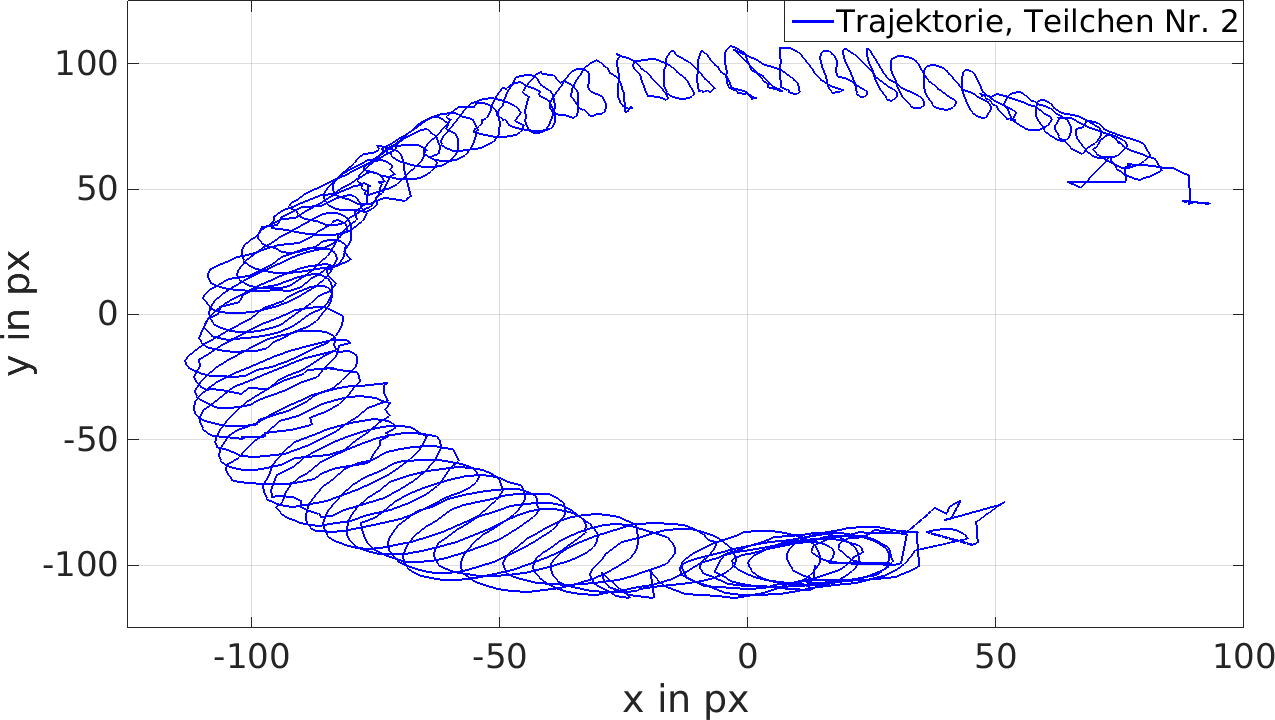
\includegraphics[width=\textwidth,height=0.8\textwidth]{figs/auswertung/gyratauszuglang.png}
              \caption{}\label{img:kreisbahn}
            \end{subfigure}
            \begin{subfigure}{0.49\textwidth}
              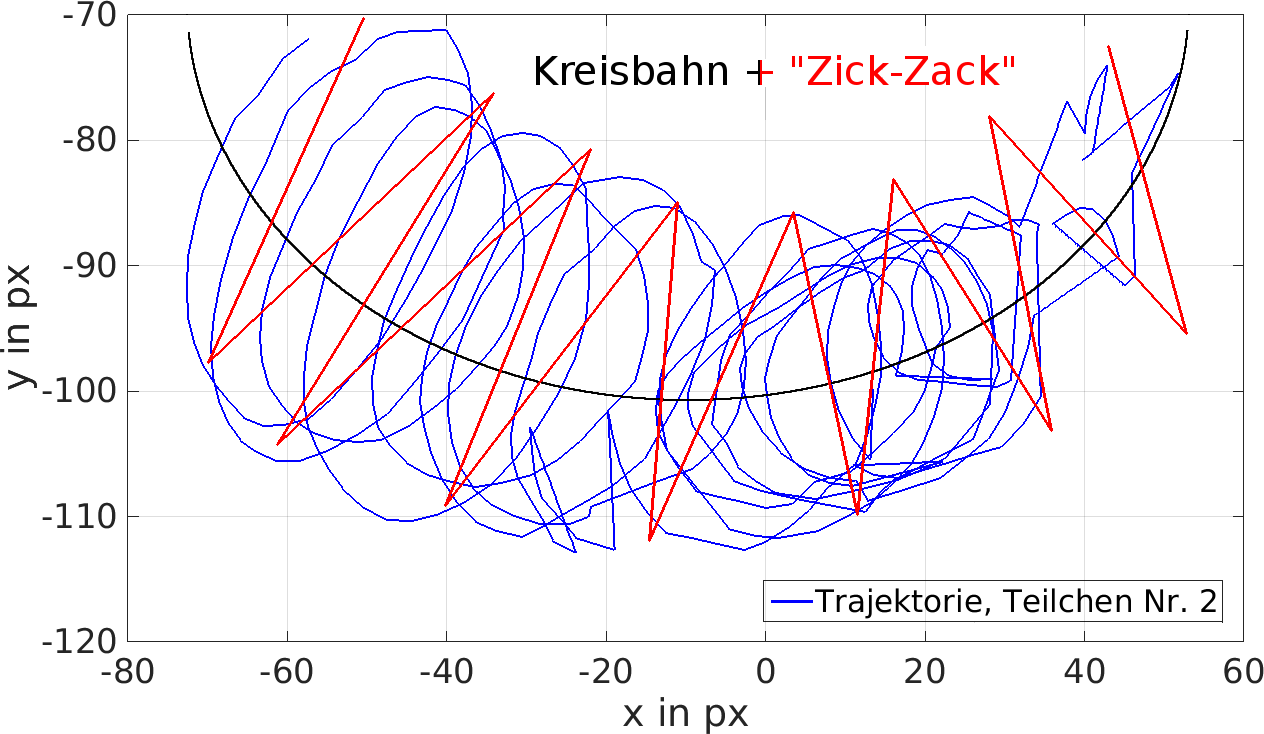
\includegraphics[width=\textwidth,height=0.8\textwidth]{figs/auswertung/gyratkurzerauszug.png}
              \caption{}\label{img:trajektorienvergleich}
            \end{subfigure}
            \caption{In \fett{(a)} die gesamte Bahn eines Teilchens auf die xy-Ebene projeziert. Die Kreisbewegung entsteht durch die Überlagerung von Gyration und Translation. Die Abbildung \fett{(b)} zeigt den Vergleich des Verlaufes der Anregung und tatsächlichen Trajektorie.}
          \end{figure}

\newpage

            \begin{figure}[!h]
              \centering
              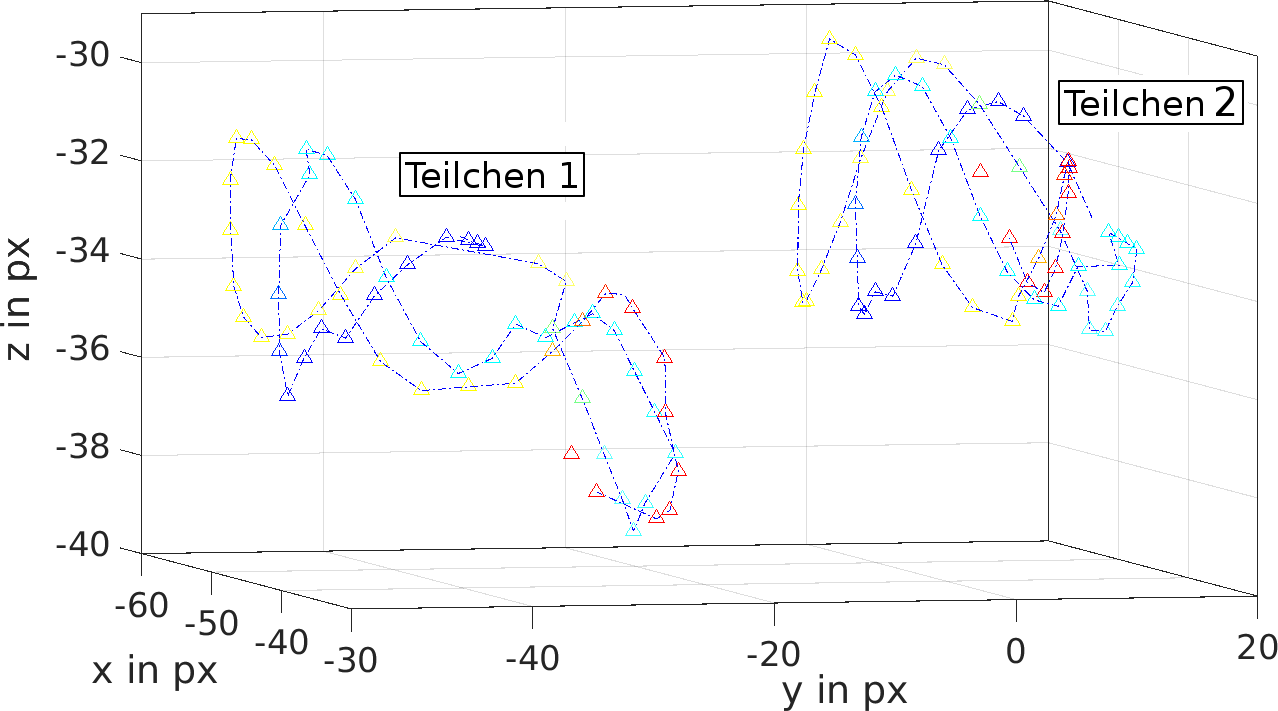
\includegraphics[width=0.7\textwidth]{figs/auswertung/gyratcoloredeins.png}
              \caption{Eine Perspektive für die verkürzten (etwa $\unit[1,5]{s}$) Bahnen von 2, auf einer Schale aufeinander folgende Partikel. Das Teilchen 1 entspricht dem aus \autoref{img:trajektorienvergleich} usw., wobei es sich bei der Cluster-Konfiguration um die aus \autoref{img:volltraj} handelt. Der zeitliche Verlauf der Bewegung ist durch die Farben der Messpunkt-Dreiecke kodiert. Die Bahn beginnt bei Blau und endet bei Rot.}\label{img:perspekt1}
            \end{figure}

            \begin{figure}[!h]
              \centering
              \includegraphics[width=0.7\textwidth]{figs/auswertung/gyratcoloredzwei.png}
              \caption{Analoge Darstellung zu \autoref{img:perspekt1}, nur aus einer anderen Perspektive. Die extremalen vertikalen Auslenkungen finden sich in den Umkehrpunkten der Gyration. Dabei ist das Teilchen für einen minimalen Radius (in Bezug auf die Ring-Mitte) am tiefsten und für einen maximalen am höchsten.}\label{img:perspekt2}
            \end{figure}

          Die Bahnen, wie sie besonders gut \autoref{img:perspekt2} zeigt, wurden in diesem Versuch vermutlicher Weise das erste mal beobachtet. Dieses Phänomen könnte unter Umständen gezielt genutzt werden, um viel Energie in das Yukawa-System zu bringen und damit einen Phasenübergang zu erzwingen. Die Idee dazu ist, dass mit der Gyration eine zusätzliche Bewegung der Teilchen den Cluster stärker aufheizt und die Energie in diesem bis zur Auflösung seiner charakteristischen Struktur erhöht.\\
          Interessant ist zudem, dass bei genauerem Analysieren der vorherigen Abbildungen ein leichter \tilt{off-set} in der Höhe zwischen den beiden Teilchen besteht. Außerdem haben deren Gyrations-Radien eine ebenso signifikante Differenz. Diese Unterschiede könnten durch kleine Variationen der Partikel-Ausdehnung, Ladung und lokalen Felder hervorgerufen werden. Demnach würde sich eine Untersuchung der Struktur und Beschaffenheit des Clusters auf Grundlage dieser Daten anbieten. Eine tiefer greifende Beschreibung dieser Erscheinung zählt zu den Ausblicken der Arbeit.

\newpage

  \section{Zusammenfassung und Ausblick}

    Mit Erfolg konnten, im Rahmen dieser Arbeit, gezielte Manipulationen von finiten Yukawa-Systemen vorgenommen werden. Dabei gelang die Anregung von Schwingungen entlang fester (orthogonaler) Achsen (Dipol, Quadrupol) besonders gut. Das ursprüngliche Ziel, mit Hilfe der Ring-Elektroden selektierte, komplexere Moden (Octopol,Hexapol) anzuregen, konnte jedoch nur partiell erfüllt werden. Probleme ergaben sich zum Beispiel bei der Konzeption und Herstellung der komplizierten Einfang-Hilfen: je mehr Symmetrie-Achsen diese besaßen, umso schwieriger gestaltete sich die Signal-Übertragung auf die Segmente. Des Weiteren war die Abstimmung der einzelnen Schwingungsachsen aufeinander und die Justierung der Manipulation im Sinne gleicher Amplituden ein Hindernis. Besonders auf Grund der Randschicht-Veränderung durch die Befestigung der Ring-Elektrode wurde die Symmetrie der verschiedenen Messungen gestört (siehe Abschnitt \ref{sub:glowanalys}). Eine Fortsetzung der Versuche dieser Arbeit könnte mit der Konstruktion besserer Elektroden beginnen. \\
    Die Aufgabe, Ergebnisse aus zBsp. \cite{Mulsow13} hinsichtlich der Eigenmoden der Dipol- und Quadrupol-Schwingung nachzuvollziehen und für die Kupfer-Ringe zu bestätigen, sowie damit deren Anwendung zu rechtfertigen, wurde erfolgreich gelöst. Demnach ist es gelungen, die Anregung einer Fluidmode (Quadrupol) in Normal-/Eigenmoden (aus \autoref{eq:ewp}) auszudrücken (Abschnitt \ref{sec:manip}) und somit deren Äquivalenz zu zeigen. Die Aufnahme der Gyrations-Bahnen aus Abschnitt \ref{sub:gyrat} eröffnet eine neue Perspektive der Aufheizung des Clusters. Weiterführende Untersuchungen diesbezüglich könnten neue Informationen über die Zusammenhänge der Phasen eines finiten Yukawa-Systems ergeben.\\
    Die Beobachtung der Schwingungs-Antworten eines Clusters waren sehr interessant und aufschlussreich für das Verständnis der Dynamik. Hier konnte, auf Grund der Übereinstimmung der Ergebnisse aus den Abschnitten \ref{subsec:phasenanal} und \ref{sec:manip}, nochmals der Zusammenhang zwischen Fluid-Beschreibung und Normalmoden-Analyse nachvollzogen werden.\\
    Die Untersuchungen zur Randschicht innerhalb der Ring-Elektrode erfüllten ihre Funktion als Fehlerbetrachtung sehr gut: aus der Analyse des Glow konnten viele Informationen über die Beschaffenheit der Segmente und die Verläufe der Anregungen am/im Ring gewonnen werden. Die Entdeckung der Randschicht-Oszillationen in der Mitte ist dabei das herausstechendste Ergebnis. Ein diesbezüglich vertiefendes Experiment könnte sich mit den expliziten Dichten und Potentialen der nahen Randschicht um ein solches Objekt während ähnlicher Analysen auseinandersetzen.\\
    Da mit der Entwicklung, dem Bau und der Implementierung eigener Komponenten für dieses Experiments dem grundlegenden Ablauf - von der Idee bis zur Umsetzung - wissenschaftlichen Arbeitens nachgegangen wurde, gehen die Ergebnisse dieser Arbeit über die, der auf Papier festgehaltenen hinaus. Insbesondere die Arbeit und Einblicke während des Aufbaus um die Plasma-Kammer, wie sie in \autoref{img:photo} gezeigt ist, haben viele Erfahrungen mit sich gebracht.

  \bibliography{all_melzer2.bib}
  \bibliographystyle{unsrt}

